\documentclass{article}
\usepackage{iclr2027_conference,times}
\usepackage{amsmath,amssymb,amsthm,bm}
\usepackage[hidelinks]{hyperref}
\usepackage{url}
\usepackage{booktabs}
\usepackage{graphicx}
\usepackage{array}
\usepackage{float}
\usepackage{needspace}
\usepackage[section]{placeins}

\theoremstyle{plain}
\newtheorem{theorem}{Theorem}
\newtheorem{proposition}{Proposition}
\newtheorem{corollary}{Corollary}
\newtheorem{lemma}{Lemma}

\title{Why Weak Features Hide:\\ The Detector Axis Hole Is Not a Free-Decoder Constraint}

\author{Anonymous authors\\Paper under double-blind review}

\newcommand{\Wihat}{\widehat{W}_i}
\newcommand{\sigeff}{\sigma_{\mathrm{eff}}}
\newcommand{\Mind}{\mathcal{M}_{\mathrm{ind}}}

\begin{document}
\maketitle
\lhead{Under review as a conference paper at ICLR 2027}

\begin{abstract}
 A weak feature can be invisible to a feature-independent test when coordinate-wise nuisance absorbs its covariance spike. We derive the local visibility coefficient $1-\lVert \Wihat\rVert_4^4$ and show that the resulting axis hole belongs to the detector class, not to an unconstrained sparse-decoder representation. In a pre-specified matched-strength TopK control, independence power is $0.081$ for an axis feature and $1.000$ for a dense feature, while both geometries meet the frozen recovery criterion in all eight seeds. A held-out excess-risk identity gives a target-alignment certificate for any frozen decoder subspace. Under matched compute, a training-only spectral warm start raises synthetic recovery from $23/48$ to $44/48$ and from $39/96$ to $89/96$ on independent fresh seeds. On real WikiText residual backgrounds, recovery changes from $28/48$ to $31/48$ for GPT-2 and from $21/48$ to $38/48$ for Pythia, without a detectable held-out reconstruction cost. A separate Pythia-160M layer-$6$ extension changes recovery from $28/48$ to $33/48$ with a cosine gain of $0.034$, but increases held-out MSE by $0.000665$. These results support a detector-class boundary and a conditional positive construction, not a universal recovery theorem for unconstrained SAEs.
\end{abstract}

\section{Introduction}
\label{sec:intro}

Sparse autoencoders leave a residual floor~\citep{gao2025scaling,engels2025dark}. One tempting account is geometric: a weak feature aligned with a coordinate axis is absorbed by coordinate-wise variance, so a present feature can be invisible. That account is true of a \emph{fixed-basis independence test}. It does not follow from the model class of an unconstrained sparse decoder. Unlabeled linear reconstruction faces a quartic sample bound, $N^\star\asymp\lambda^{-4}$; a conditional isolation stage recovers the labeled quadratic bound once a separating direction is available. The measured TopK results follow these strength-dependent benchmarks. Neither bound has an axis hole.

Superposition lets many features share a low-dimensional representation~\citep{elhage2022toy,scherlis2023polysemanticity}. SAEs are the practical tool for separating them~\citep{cunningham2024sae,bricken2023towards,gao2025scaling}, but residuals, absorption, multi-dimensionality, and seed dependence persist~\citep{engels2025dark,chanin2024absorption,engels2024nonlinear,leask2025canonical}. Before assigning a miss to optimization or semantics, we ask which evidence channel disappeared.

A detector class is a statistic together with the nuisance parameters it may refit. Labels use a mean ($N^\star\asymp\lambda^{-2}$). Fixed-background covariance uses the full second-order spike ($N^\star\asymp\lambda^{-4}$). A feature-independent detector further drops the diagonal and multiplies the quartic rate by $1-\lVert \Wihat\rVert_4^4$. Unconstrained dictionary learning can place an atom on any direction, including an axis, so that last factor is not an SAE coefficient. Reconstruction rates follow the encoder, not $\Mind$: a linear encoder is quartic uniformly in $w$; a conditional isolating encoder is quadratic uniformly in $w$ after a separating direction is available. The experiments isolate the distinction: rotate the basis and only the independence statistic moves; sweep $\lambda$ and SAE recovery is strength-dependent in both geometries.

Our claim boundary is deliberately narrow: the coefficient is a property of a fixed-basis independence test, not a representation-level constraint on free sparse decoders. We contribute (i) a nuisance-projection calculus and whitened quartic law, (ii) a matched detector--TopK control separating detector visibility from free-SAE recovery, (iii) a conditional held-out certificate, and (iv) a matched-compute spectral initialization that improves recovery across objectives and capacities, replicates on fresh seeds, and transfers with model-dependent effect size to two real residual backgrounds. The exact anchor-preserving theorem remains a structured positive family with explicit data--target linkage, not a theorem about unconstrained SAE training.

\section{Related work}
\label{sec:related}

SAEs recover interpretable directions at scale, but residual floors, absorption, and non-canonical atoms persist~\citep{cunningham2024sae,bricken2023towards,gao2025scaling,engels2025dark,chanin2024absorption,leask2025canonical}. Superposition and dictionary-learning work study overcomplete representations and global recovery~\citep{elhage2022toy,scherlis2023polysemanticity,spielman2012exact,arora2014new}; spiked-covariance theory studies spectral thresholds~\citep{johnstone2001distribution,baik2005phase,cai2013sparse,berthet2013complexity}. We instead quantify the evidence lost when a specified nuisance family refits diagonal variance, using local testing and projection~\citep{lecam1986asymptotic,amari2000methods,bickel1993efficient}.

\section{Preliminaries}
\label{sec:prelim}

\paragraph{Dark matter as a detectability floor.}
SAE scaling usually lowers reconstruction error without driving it to zero~\citep{gao2025scaling,engels2025dark}. Empirically, dark matter is unexplained representation variance. We give a feature-level statistical definition: it is the variance carried by features that are present but fall below the detection boundary of the decoder class. The two definitions coincide when detectability is the binding constraint. They diverge when optimization, absorption, or nonlinearity dominate.

\paragraph{Superposition model.}
Let $n$ latent features share an $m$-dimensional representation with $n\gg m$. The linear encoding is $h=Wx+\sigma\varepsilon$, where $W=[W_1,\ldots,W_n]\in\mathbb{R}^{m\times n}$, $\varepsilon\sim\mathcal{N}(0,I_m)$, and $\sigma>0$. Feature $i$ activates with probability $p_i$ along $W_i$. Let $\nu_i$ denote its centered second moment; $\nu_i=p_i(1-p_i)$ and $\nu_i\approx p_i$ when rare. The representation covariance is
\begin{equation}
\Sigma_h=\sigma^2 I_m+\sum_{i=1}^n \nu_i W_i W_i^{\top}.
\end{equation}
The scalar $\lambda_i:=\sqrt{\nu_i}\,\lVert W_i\rVert$ is the effective strength of feature $i$. If a decoder fails to recover feature $i$, the variance $\nu_i\lVert W_i\rVert^2$ remains in the residual.

\paragraph{Feature recovery as testing.}
Fix a feature index $i$. Given $N$ independent samples $h^{(1)},\ldots,h^{(N)}$, test
\begin{equation}
H_0^{(i)}:\ \Sigma_h=\sigma^2 I_m+\sum_{j\neq i}\nu_j W_j W_j^{\top},
\qquad
H_1^{(i)}:\ \Sigma_h=\sigma^2 I_m+\sum_{j=1}^n \nu_j W_j W_j^{\top}.
\end{equation}
Let $N_i^*$ be the smallest sample size at which this test achieves vanishing error probability. In the labeled setting the detector sees the activation indicator and exploits a first-order mean shift, yielding $N_i^*\asymp\lambda_i^{-2}$. In the unlabeled setting the perturbation $\nu_i W_i W_i^{\top}$ enters at second order, so a covariance detector against a \emph{fixed} background faces $N_i^*\asymp\lambda_i^{-4}$. Standard SAEs encourage sparse independent latents~\citep{bricken2023towards,gao2025scaling}, so a feature-independent background is the natural \emph{test} null and can absorb the diagonal, introducing $1-\lVert \Wihat\rVert_4^4$. Reconstruction, the SAE \emph{training} objective, is not that test: Theorem~\ref{thm:recon} gives $\lambda^{-4}$ for a linear encoder and a conditional $\lambda^{-2}$ isolation benchmark once a separating direction is available, both without the axis coefficient.

\section{A local detector-class visibility calculus}
\label{sec:calculus}

\subsection{Local Gaussian covariance slice}
Write $\Sigma_h=\Sigma_{-i}+\nu_i W_i W_i^{\top}$ with $\Sigma_{-i}$ the background from all features except $i$. We analyze the weak-feature regime under the local isotropy reduction $\Sigma_{-i}\approx\sigeff^2 I_m$, where $\sigeff^2=\sigma^2+m^{-1}\sum_{j\neq i}\nu_j\lVert W_j\rVert^2$. This does not claim that the background is isotropic at every scale; it says that, at the scale relevant for detecting a weak feature, the aggregate background can be summarized by an effective per-dimension variance. After this reduction,
\begin{equation}
H_0^{(i)}:\ h\sim\mathcal{N}(0,\sigeff^2 I_m),\qquad
H_1^{(i)}:\ h\sim\mathcal{N}\bigl(0,\sigeff^2 I_m+\lambda_i^2 \Wihat\Wihat^{\top}\bigr),
\end{equation}
where $\Wihat:=W_i/\lVert W_i\rVert$.

\subsection{Projection calculus}
\begin{proposition}[Detector-class projection]
\label{prop:proj}
Let $\mathcal{M}_D$ be the regular background family that detector class $D$ may refit, with score tangent space $T_D$ at $P_0=\mathcal{N}(0,s^2 I_m)$. In the local Gaussian covariance slice, for $P_\lambda=\mathcal{N}(0,s^2 I_m+\lambda^2 ww^{\top})$ and $\psi_w(h)=((w^{\top}h)^2-s^2)/(2s^4)$,
\begin{equation}
\inf_{Q\in\mathcal{M}_D} D_{\mathrm{KL}}(P_\lambda\Vert Q)=\frac{\lambda^4}{2}\bigl\lVert \psi_w-\Pi_{T_D}\psi_w\bigr\rVert_{L^2(P_0)}^2+O(\lambda^6).
\end{equation}
\end{proposition}
Feature visibility is the squared norm of the feature score after quotienting out the nuisance directions available to the detector. The proof is in Appendix~\ref{app:proj}.

\subsection{Feature-independent background}
\label{sec:coords}
SAE-like decoders operate against a background that treats contributions as independent and therefore refits coordinate-wise variances rather than arbitrary correlations. We represent this local model class by the diagonal Gaussian family
\begin{equation}
\Mind:=\bigl\{\mathcal{N}\bigl(0,\mathrm{diag}(d_1,\ldots,d_m)\bigr):d_j>0\bigr\}.
\end{equation}
This diagonal null is a local analytic proxy for feature-independence, not a claim that GPT-2 activations or trained SAEs factorize coordinate-wise. Its role is to encode which nuisance directions the detector may refit. It can absorb diagonal variance inflation but cannot create new off-diagonal correlations.

\paragraph{Which coordinates?}
The diagonal model is defined in a specified orthonormal frame $B$. In the synthetic experiments below, $B=I$. In the GPT-2 bridge, $B$ is the train-split PCA whitening map. Axis-aligned means $B^{\top}w=e_j$ in \emph{that} frame, not that semantic features are intrinsically neuron-aligned, and not that SAE decoder atoms are aligned with PCA axes. If the nuisance tangent space is transformed, the blind spot moves with it. Section~\ref{sec:exp} rotates $B$ while holding $\lambda$ fixed; the ind detector follows $1-\lVert B^{\top}w\rVert_4^4$, while labels do not.

Let $s^2=\sigeff^2$, $w=\Wihat$, and $t=\lambda_i^2/s^2$. The best diagonal null matches the diagonal of the spiked covariance, so the trace term cancels and only the off-diagonal residual remains. Equivalently, $ww^{\top}=\mathrm{diag}(w_1^2,\ldots,w_m^2)+R_w$ and only $R_w$ is normal to the tangent space, with $\lVert R_w\rVert_F^2=1-\lVert w\rVert_4^4$.

\begin{theorem}[Quartic law under a feature-independent background]
\label{thm:quartic}
Under the local isotropy reduction above, the minimum local KL divergence between the alternative in $H_1^{(i)}$ and $\Mind$ satisfies
\begin{equation}
D_{\mathrm{loc}}^{(i)}(\lambda_i)=C_i\lambda_i^4+O(\lambda_i^6),\qquad
C_i=\frac{1-\lVert \Wihat\rVert_4^4}{4\sigeff^4}.
\end{equation}
When $C_i>0$, the sample complexity is $N_i^*\asymp C_i^{-1}\lambda_i^{-4}$. If $C_i=0$, the diagonal family absorbs the spike at this order; in the exactly coordinate-aligned case the KL gap is identically zero.
\end{theorem}

\begin{corollary}[Whitened form]
\label{cor:white}
For a general background $\Sigma_{-i}\succ 0$, set $\tilde h=\Sigma_{-i}^{-1/2}h$, $\tilde w=\Sigma_{-i}^{-1/2}W_i/\lVert\Sigma_{-i}^{-1/2}W_i\rVert$, and $\tilde\lambda_i:=\sqrt{\nu_i}\lVert\Sigma_{-i}^{-1/2}W_i\rVert$. In the whitened coordinates the same diagonal nuisance yields $D_{\mathrm{loc}}^{(i)}=(1-\lVert\tilde w\rVert_4^4)\tilde\lambda_i^4/4+O(\tilde\lambda_i^6)$. The exponent is unchanged; both strength and geometry are evaluated after whitening. Local isotropy is the special case $\Sigma_{-i}=\sigeff^2 I_m$, where $\tilde\lambda_i=\lambda_i/\sigeff$.
\end{corollary}

A two-dimensional toy makes the geometry concrete. For $m=2$, $w=(1,0)$ has $C=0$; $w=(1/\sqrt{2},1/\sqrt{2})$ has $C=1/2$. At the same $\lambda$ and $N$, the first feature has $E_{\mathrm{ind}}=0$ at this order and the second has $E_{\mathrm{ind}}\asymp N\lambda^4/2$. Equal strength is not equal evidence. Figure~\ref{fig:scheme} shows what each class keeps.

\begin{figure}[ht]
\centering
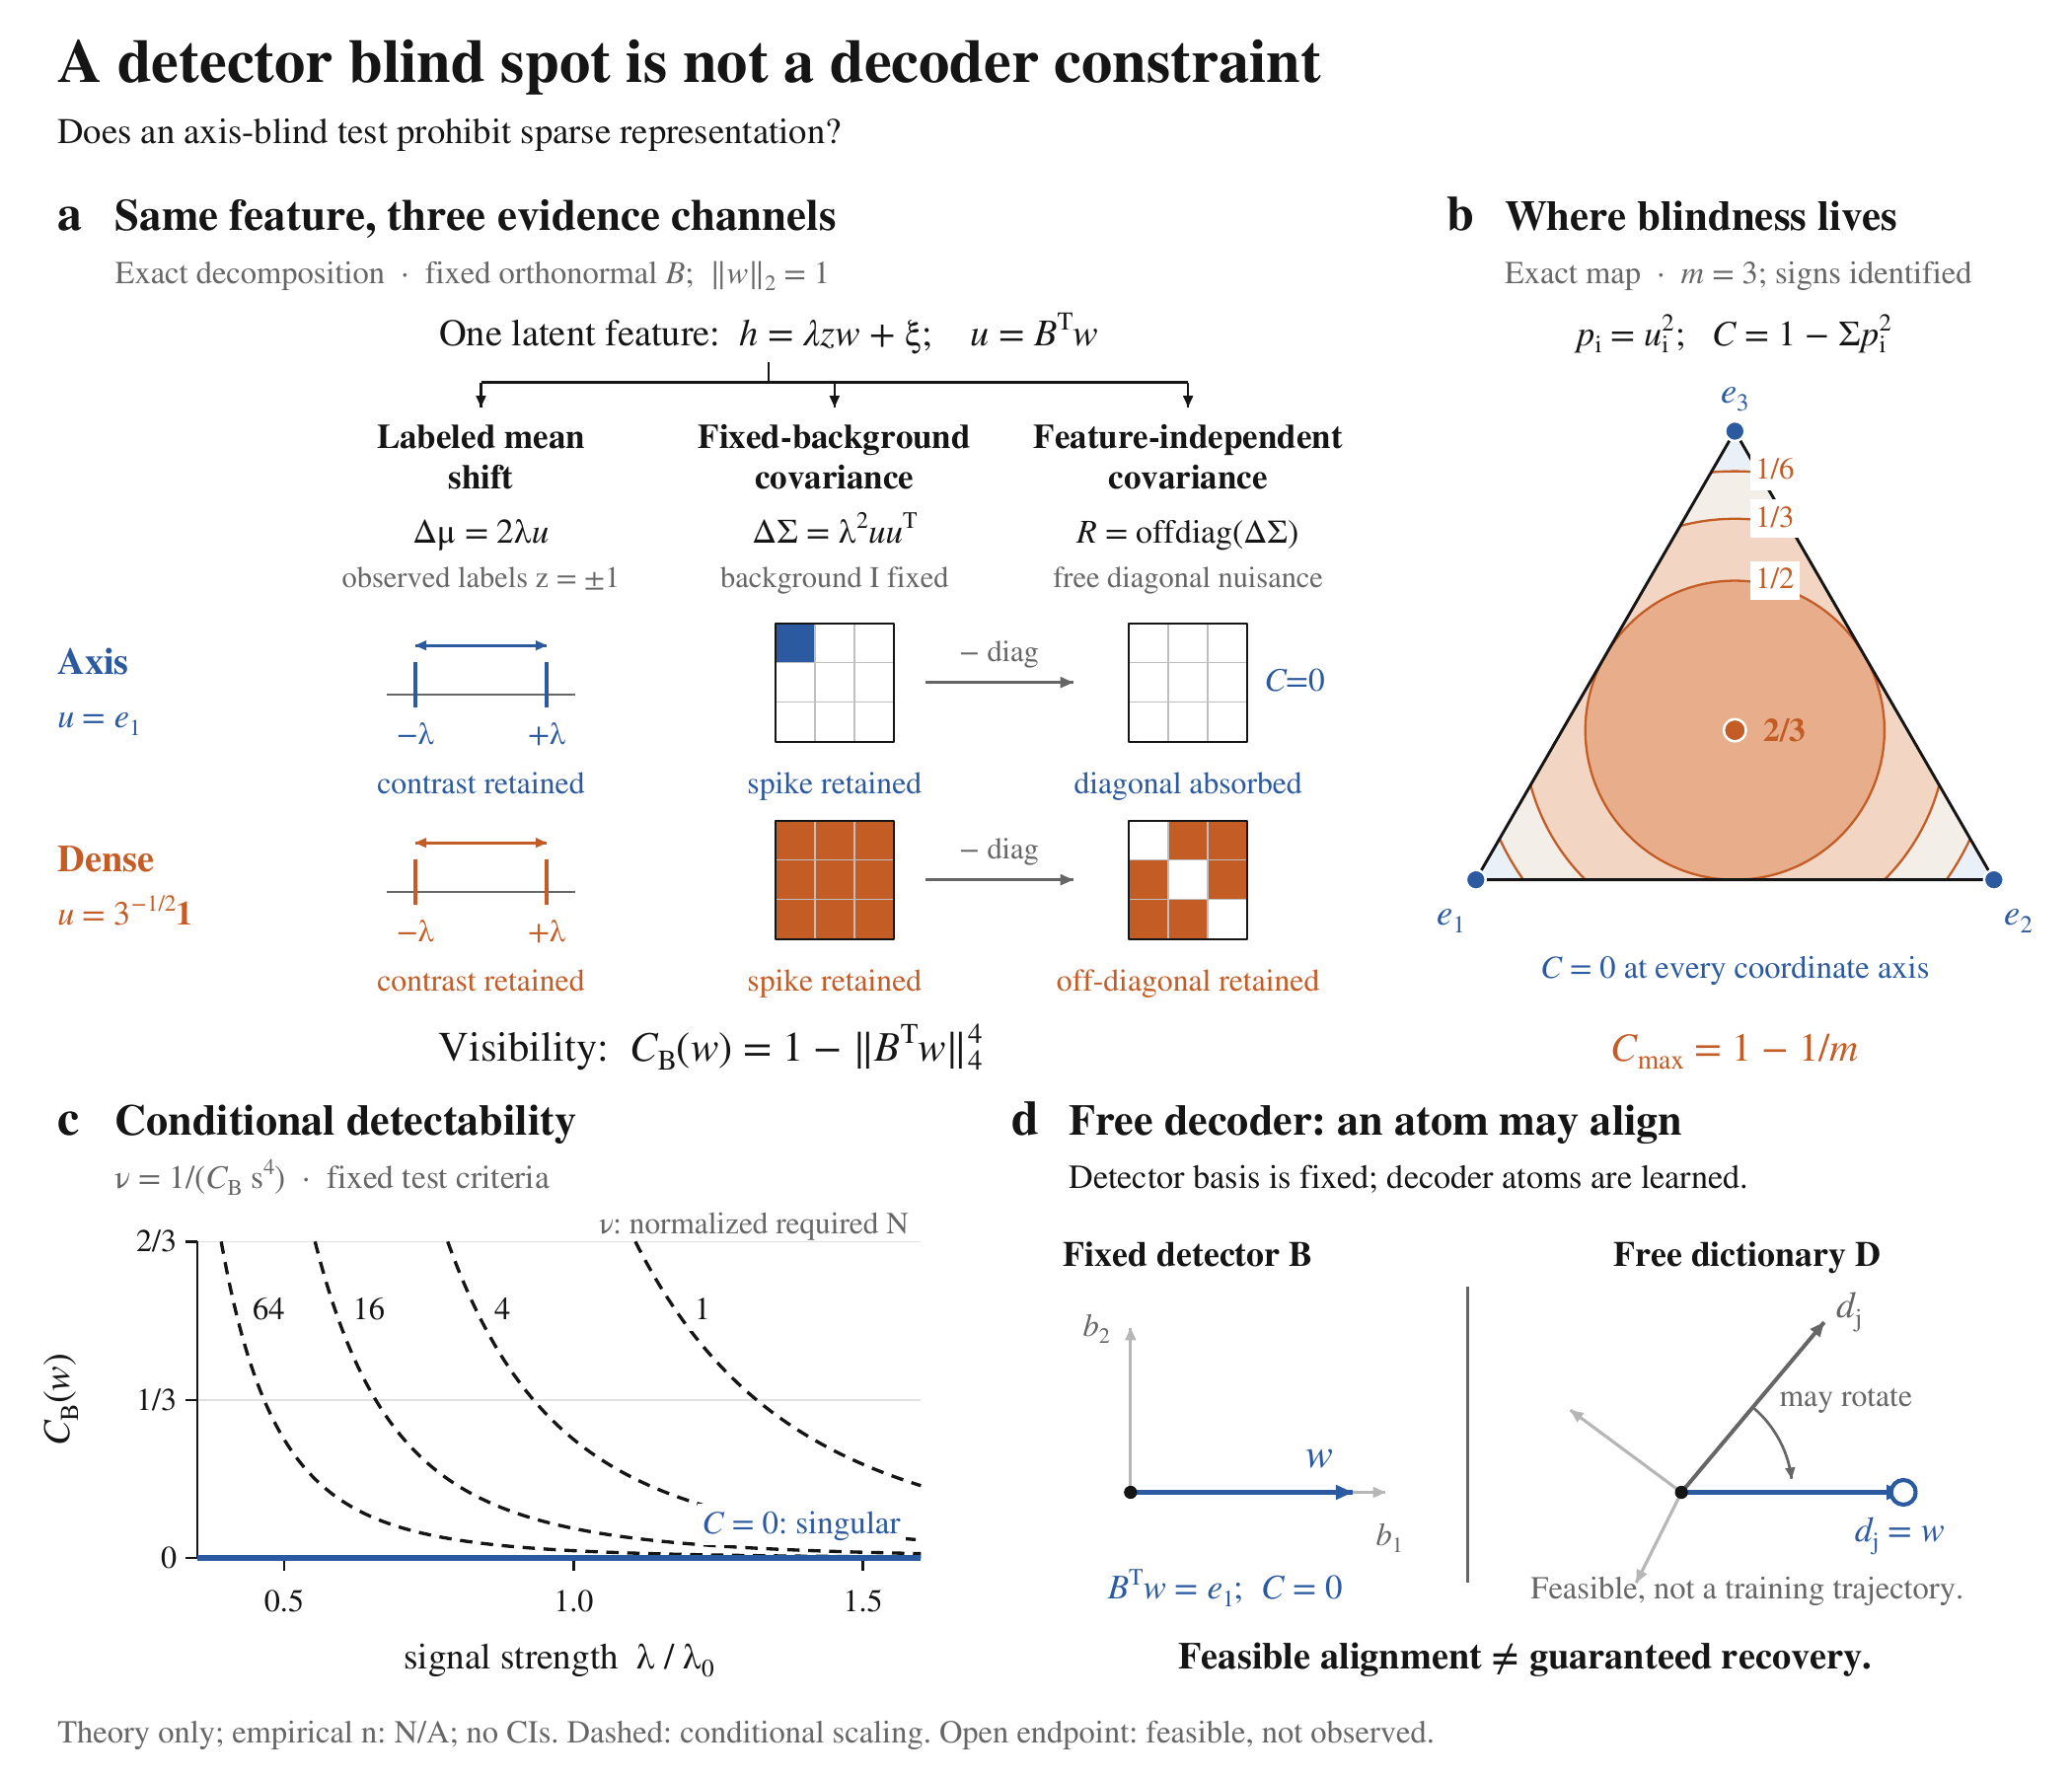
\includegraphics[width=\linewidth]{figures/fig1_detector_boundary.png}
\caption{\textbf{A detector blind spot is not a decoder constraint.} \textbf{(a)} For the same feature, labels retain a mean contrast, fixed-background covariance retains the full rank-one spike, and a feature-independent covariance test retains only its off-diagonal part. \textbf{(b)} The visibility coefficient $C_B(w)=1-\lVert B^\top w\rVert_4^4$ vanishes on the detector axes and is maximized by a dense loading. \textbf{(c)} Conditional sample requirements diverge as $C_B(w)\to0$. \textbf{(d)} A free decoder can represent an axis direction, but feasibility alone is not a training or recovery guarantee. Panels (a--d) are theoretical schematics; they contain no empirical observations or confidence intervals.}
\label{fig:scheme}
\end{figure}

\subsection{Detector-class hierarchy}
\begin{corollary}[Feature visibility principle]
\label{cor:vis}
Up to constants and slowly varying thresholds,
\begin{equation}
E_{\mathrm{label}}(i)\asymp N\lambda_i^2,\qquad
E_{\mathrm{cov}}(i)\asymp N\lambda_i^4,\qquad
E_{\mathrm{ind}}(i)\asymp N\bigl(1-\lVert \Wihat\rVert_4^4\bigr)\lambda_i^4.
\end{equation}
\end{corollary}

\begin{corollary}[Detector-class hierarchy]
\label{cor:hier}
In the weak-signal limit, $E_{\mathrm{label}}(i)\ge E_{\mathrm{cov}}(i)\ge E_{\mathrm{ind}}(i)$. If $\Wihat=e_j$ in the detector coordinates, then $E_{\mathrm{ind}}=0$ at leading quartic order, while labels and fixed-background covariance still see the feature.
\end{corollary}

If the feature were absent, all three tests would fail. If the covariance spike existed but were not absorbed, cov and ind would agree. The distinctive prediction is a detector-class split: present, label-visible, covariance-visible, and feature-independent-invisible.

That split is a property of $\Mind$, not a representation-level constraint on every sparse decoder.

\begin{theorem}[The axis hole is not a free-decoder constraint]
\label{thm:saeclass}
Let $\mathcal{F}_k=\{Dz:\lVert z\rVert_0\le k\}$ be a $k$-sparse linear decoder with unconstrained dictionary $D\in\mathbb{R}^{m\times d}$ and $d\ge 1$. For every unit $w$, including $w=e_j$, some $D$ and $1$-sparse $z$ realize $Dz=\alpha w$. Thus the axis direction is available to the decoder class even when $C_{\mathrm{ind}}=0$; the fixed-basis independence coefficient is not a constraint on this model class. This is a representation statement, not a claim about optimization or about projecting probability models onto $\mathcal{F}_k$.
\end{theorem}

\begin{proposition}[Why a structural constraint is necessary]
\label{prop:unconstrained_no_bound}
Let $m\ge2$, $k\ge1$, and let $\mathcal{F}_k$ be the unconstrained $k$-sparse decoder class above. Membership in $\mathcal{F}_k$ alone gives no positive uniform alignment bound: for every unit target $w$, there is a feasible decoder whose active atom is any prescribed unit vector $v$, including one with $v\perp w$, so its target alignment is zero. This is a statement about the feasible model class, not about every learning procedure: it does not rule out a data-dependent algorithm that uses samples to select $v$. A positive recovery theorem therefore needs an explicit data--target linkage assumption, such as the training-only spectral anchor and anchor-preserving constraints used below.
\end{proposition}

\begin{theorem}[Objective-agnostic reconstruction certificate]
\label{thm:certificate}
Let $X$ be centered with covariance $\Sigma=\sigma^2 I_m+\tau ww^{\top}$, where $\tau>0$ and $\lVert w\rVert=1$. Let $P$ be the orthogonal projector onto any rank-$r$ decoder subspace, and let $P_w$ be any rank-$r$ projector whose range contains $w$. Define $R(P)=\mathbb{E}\lVert X-PX\rVert^2$. Then
\begin{equation}
R(P)-R(P_w)=\tau\bigl(1-\lVert Pw\rVert^2\bigr)=\tau\sin^2\!\angle(w,\operatorname{range}P).
\end{equation}
Consequently, for any objective, optimizer, initialization, or decoder parameterization that produces $P$, an independent validation estimate $\widehat\Delta$ of this excess risk yields the certificate $\cos\angle(w,\operatorname{range}P)\ge\sqrt{1-\widehat\Delta/\tau}$ whenever $0\le\widehat\Delta\le\tau$. If $X$ is Gaussian and the validation set has $n$ samples, then with probability at least $1-\delta$ one may replace $\widehat\Delta$ by $\widehat\Delta+\epsilon_{n,r,\delta}$, where
\begin{equation}
\epsilon_{n,r,\delta}=2(\sigma^2+\tau)\left(\sqrt{\frac{4r\log(2/\delta)}{n}}+\frac{\log(2/\delta)}{n}\right).
\end{equation}
The certificate is objective-agnostic but conditional on the rank, covariance model, target-specific oracle comparison, and independent validation split; it is not an optimization or unknown-direction discovery guarantee.
\end{theorem}

\begin{theorem}[Objective/capacity-uniform spectral-anchor recovery]
\label{thm:spectral_anchor}
Let $X_1,\ldots,X_N$ be independent centered Gaussian samples with covariance $\Sigma=\sigma^2 I_m+\tau ww^{\top}$, where $\tau>0$ and $\lVert w\rVert=1$. Let $\widehat u$ be the leading unit eigenvector of the training second moment $S=N^{-1}\sum_i X_iX_i^{\top}$, with its sign fixed by a deterministic coordinate convention. If $\lVert S-\Sigma\rVert_{\mathrm{op}}\le\epsilon<\tau/2$, then $\sin\angle(\widehat u,w)\le\epsilon/(\tau-\epsilon)$. Construct a signed anchor pair $\{\widehat u,-\widehat u\}$ and restrict every residual decoder column to $\widehat u^\perp$, reserving one active TopK slot for the signed anchor. Then, for all anchor-preserving objectives and capacities, and for every optimizer and initialization that preserves these constraints, the anchor recovery is identical and satisfies\[\cos\angle(\widehat u,w)\ge\sqrt{1-\bigl(\epsilon/(\tau-\epsilon)\bigr)^2}.\] With the Gaussian-Wishart bound $\epsilon=\|\Sigma\|_{\mathrm{op}}(2q+q^2)$, $q=(\sqrt m+\sqrt{2\log(2/\delta')})/\sqrt N$, and a family-wise allocation $\delta'=\delta/G$ over $G$ training anchors, this holds simultaneously with probability at least $1-\delta$. This is a theorem for the anchor-preserving family, not for unconstrained SAE training or unknown-direction discovery.\end{theorem}

\begin{theorem}[Bounded-drift spectral-anchor recovery]
\label{thm:bounded_drift_anchor}
Let $\widehat u_0$ be the training-only leading-eigenvector anchor in Theorem~\ref{thm:spectral_anchor}, and let $\widehat u$ be a trainable unit anchor satisfying $\angle(\widehat u,\widehat u_0)\le\rho$. Allow each unit residual decoder column $v_j$ to have bounded anchor leakage $|v_j^\top\widehat u|\le\eta<1$. If the spectral estimate obeys $\sin\angle(\widehat u_0,w)\le s<1$ and $\arcsin(s)+\rho<\pi/2$, then, for all bounded-drift anchor-preserving objectives and capacities, and for every optimizer and initialization that enforces these constraints,\[\cos\angle(\widehat u,w)\ge\cos\bigl(\arcsin(s)+\rho\bigr).\] The residual leakage cap $\eta$ may be nonzero and does not weaken this anchor bound. With the family-wise Gaussian-Wishart/Davis--Kahan choice $s=\epsilon/(\tau-\epsilon)$ and $\delta'=\delta/G$, the statement holds simultaneously with probability at least $1-\delta$ over $G$ training anchors.
\end{theorem}

The training objective is reconstruction, not a likelihood ratio against $\Mind$. The next theorem gives a linear-encoder rate and a conditional isolation benchmark; it does not give an end-to-end convergence theorem for trained TopK. Write $h=\varepsilon+a(z-p)w$ with $\varepsilon\sim\mathcal{N}(0,I_m)$, $z\sim\mathrm{Bern}(p)$, $\lambda=a\sqrt{p}$, and $\beta=\lambda^2(1-p)$.

\begin{theorem}[Reconstruction two-regime law]
\label{thm:recon}
Consider one-sparse reconstruction $\hat h=g(u^{\top}h)\,u$ with $\lVert u\rVert=1$.
(i)~Linear encoder $g(t)=\alpha t$: the top eigenvector $\hat u$ of the sample covariance satisfies $\mathbb{E}[\sin^2\theta]=(m-1)(1+\beta)/(N\beta^2)+O(N^{-2})$ with $\theta=\angle(\hat u,w)$, hence $N^\star\asymp\lambda^{-4}$ uniformly in $w$.
(ii)~Conditional isolation benchmark: assuming a direction $u$ that separates the mixture is already available and a threshold on $u^{\top}h$ isolates $\{z=1\}$ as $a\to\infty$, the resulting difference-of-means estimator satisfies $\mathbb{E}[\cos\theta]\approx\kappa(\kappa^2+m-1)^{-1/2}$ with $\kappa=\lambda\sqrt{(1-p)N}$, hence the isolation stage has $N^\star\asymp\lambda^{-2}$ uniformly in $w$. This is not an end-to-end trained-SAE guarantee.
Neither rate contains $1-\lVert w\rVert_4^4$.
\end{theorem}

\begin{proposition}[Oracle column is a residual mean]
\label{prop:oracle}
If code coordinate $0$ is clamped to $z-p$ and the remaining dictionary $D_{-0}$ is free, the population minimizer of decoder column $0$ is proportional to $\mathbb{E}[(z-p)(h-D_{-0}z_{-0})]$. Its alignment with $w$ is strictly less than one when the absorbed term has a nonzero component orthogonal to $w$ and the residual mean is nonzero. Thus the oracle column is conditional on fitting the rest of the dictionary; its finite-$N$ recovery cost cannot be interpreted without that stage.
\end{proposition}

Theorem~\ref{thm:saeclass} is a model-class observation rather than an optimization result; Theorem~\ref{thm:recon}(i) is the linear-encoder rate and (ii) is a conditional isolation benchmark; Proposition~\ref{prop:oracle} is why clamping $z$ is not the mean estimator. Gradient descent remains empirical (Section~\ref{sec:sae}).
\FloatBarrier

The recover-or-miss floor is a useful lower bound, not a trained-SAE identity: subcritical features contribute their variance only under the idealization that supercritical features are recovered and optimization adds no excess error. The full threshold derivation and the $80$-feature capacity control are in Appendix~\ref{app:additional_floor}; they show why residual mass above the detector floor can reflect capacity, absorption, optimization, correlation, or nonlinearity rather than an axis rule.
\FloatBarrier

\section{Experiments}
\label{sec:exp}

We compare three detectors against the same weak-feature alternative. Null thresholds are Monte Carlo at $\alpha=0.05$. Unlabeled samples are $h=\varepsilon+\lambda z w$ with $\varepsilon\sim\mathcal{N}(0,I_m)$, $z\sim\mathcal{N}(0,1)$, $m=8$, $N=1024$, $700$ trials, $8$ seeds, $\lambda=0.55$ unless noted. Bootstrap $95\%$ intervals use the seed as the unit.

\iffalse
\begin{table}[H]
\caption{Detector statistics. The cov background is $I$, never refit on $H_1$. Ind is written in a specified orthonormal frame $B$.}
\label{tab:detectors}
\begin{center}
\small
\begin{tabular}{@{}llp{0.46\linewidth}@{}}
\toprule
\textbf{Class} & \textbf{Statistic} & \textbf{Nuisance} \\
\midrule
label & mean shift along $w$ & none (activation known) \\
cov & $\lVert\widehat\Sigma-I\rVert_F$ & background frozen \\
ind & $\lVert\mathrm{offdiag}(\widehat\Sigma_B)\rVert_F$ & coordinate-wise variances in $B$ \\
\bottomrule
\end{tabular}
\end{center}
\end{table}
\fi

A protocol check for the rotation experiment is that label power stays identically $1$: only the coordinates of the ind statistic change.

\subsection{Primary matched detector--decoder control}
Figure~\ref{fig:sae_control} presents the pre-specified E4-v2 endpoint and its paired seed-by-strength audit before the secondary detector calibrations.

\begin{figure}[H]
\centering
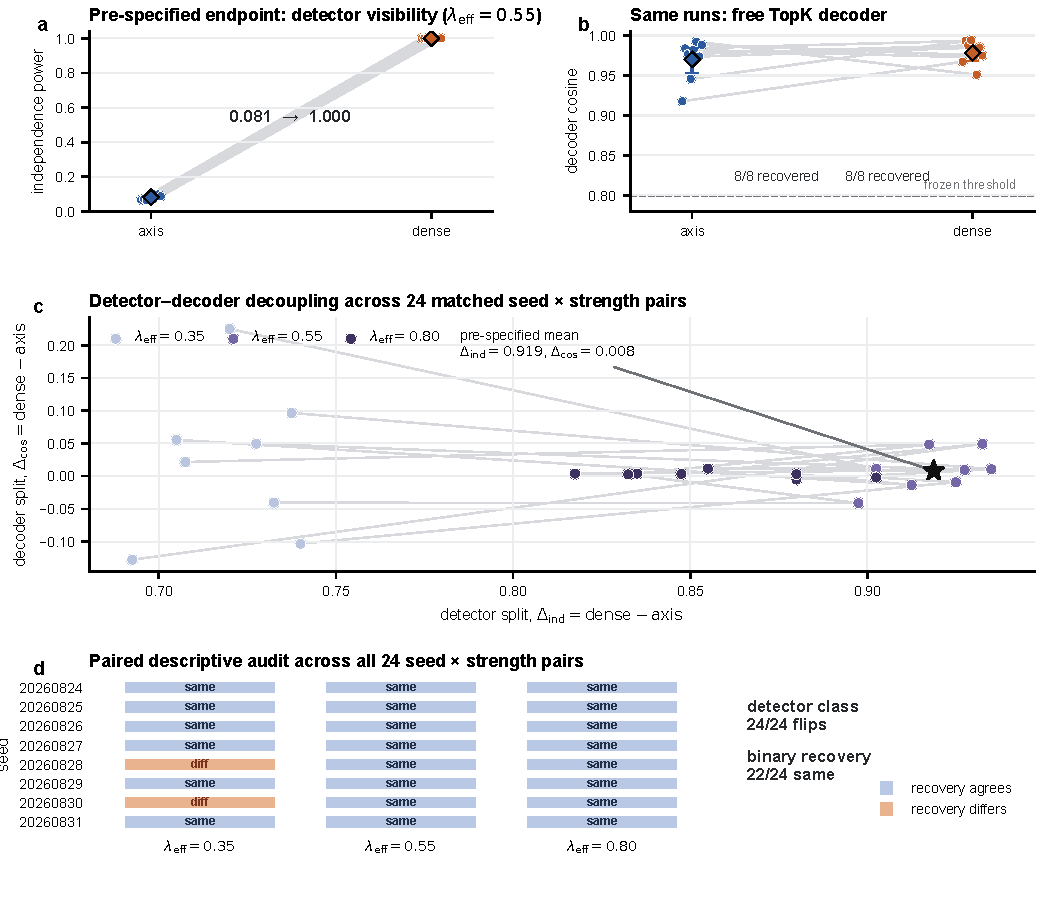
\includegraphics[width=\linewidth]{figures/fig2_detector_decoder.pdf}
\caption{\textbf{A detector-class visibility split does not transfer to matched TopK recovery.}
\textbf{a}, Pre-specified E4-v2 endpoint at $\lambda_{\mathrm{eff}}=0.55$: feature-independent detection power for axis and dense loadings. Thin lines pair the same seed across geometries; points are the eight seed-level observations, diamonds are means, and error bars are seed-level percentile-bootstrap $95\%$ confidence intervals (1,000 resamples). Power is $0.081$ $[0.073,0.090]$ for the axis loading and $1.000$ $[1.000,1.000]$ for the dense loading.
\textbf{b}, Decoder cosine from the same matched runs. Both geometries satisfy the frozen cosine-$0.80$ recovery criterion in all eight seeds (means $0.970$ and $0.978$ for axis and dense, respectively).
\textbf{c}, Detector--decoder decoupling over all 24 matched seed--strength pairs. Each point reports the dense-minus-axis difference in independence power and decoder cosine; pale trajectories connect the three strengths within a seed. The black star marks the pre-specified $\lambda_{\mathrm{eff}}=0.55$ mean ($\Delta_{\mathrm{ind}}=0.919$, $\Delta_{\mathrm{cos}}=0.008$).
\textbf{d}, Descriptive paired audit over the same 24 pairs. Detector class flips in $24/24$ pairs, whereas binary recovery status agrees in $22/24$ pairs. Panel d is descriptive rather than an additional pre-specified endpoint. The experiment uses eight seeds, $N=4096$ detector samples per trial, 400 alternative trials, a 16-atom TopK decoder with $k=2$, 20,000 training samples, and 4,000 optimization steps.}
\label{fig:detector_decoder_decoupling}

\label{fig:sae_control}
\end{figure}

\subsection{Same strength, opposite sides of the boundary}
\begin{figure}[ht]
\centering
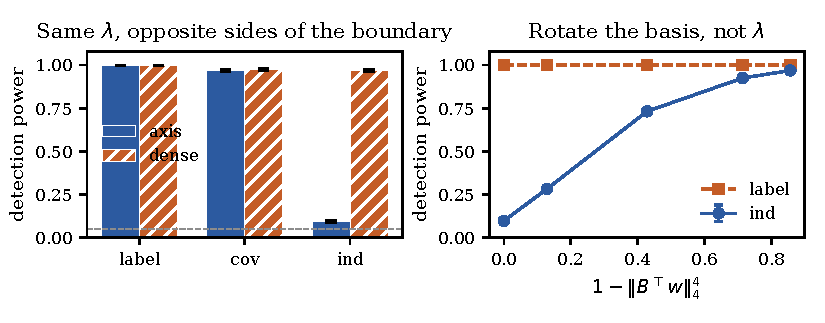
\includegraphics[width=\linewidth,height=1.45in,keepaspectratio]{figures/fig_same_lambda.pdf}
\caption{\textbf{Detector calibration.} (a) At matched $\lambda$, only the feature-independent statistic shows the axis--dense gap. (b) At fixed $\lambda$, rotating $B$ moves independence power with $1-\lVert B^{\top}w\rVert_4^4$ ($r=0.977$), while label power remains one.}
\label{fig:same}
\vspace{-0.5em}
\end{figure}

At matched $\lambda$, axis and dense features are label-visible (power $1.000$) and covariance-visible ($0.969/0.974$), but independence power is $0.096$ $[0.090,0.102]$ versus $0.969$ $[0.965,0.974]$. Rotating $B$ at fixed strength gives $r=0.977$ with label power one; the two-sparse control gives $r=0.972$ (versus $0.808$ for $\lVert u\rVert_1$). Figure~\ref{fig:same} reports the calibration.

\iffalse
\begin{table}[H]
\caption{Synthetic suite. Intervals are seed-level bootstrap $95\%$ CIs.}
\label{tab:results}
\begin{center}
\small
\begin{tabular}{@{}>{\raggedright\arraybackslash}p{0.36\linewidth}>{\raggedright\arraybackslash}p{0.56\linewidth}@{}}
\toprule
\textbf{Check} & \textbf{Result} \\
\midrule
Detector $N^\star(\lambda)$ slope (label / unlabeled) & $-1.95$ vs.\ $-3.72$ (theory: $-2$ vs.\ $-4$) \\
Same-$\lambda$ ind power & axis $0.096$ $[0.090,0.102]$; dense $0.969$ $[0.965,0.974]$ \\
Rotate $B$, hold $\lambda$ & ind vs.\ $1-\lVert B^{\top}w\rVert_4^4$: $r=0.977$; label $\equiv 1$ \\
2-sparse imbalance $\varepsilon$ & $0.123$ ($\varepsilon{=}0.01$) $\to$ $0.810$ ($\varepsilon{=}0.50$) \\
Ind recover-or-miss floor vs.\ $N$ & predicted vs.\ missed variance $r=0.999$, MAE $0.005$ \\
TopK cosine vs.\ $\lambda$ (axis / dense) & $0.85$/$0.85$ at $0.38$; $0.32$ still near chance \\
Ind power vs.\ $\lambda$ (axis / dense) & $0.058$/$0.598$ at $0.32$; $0.064$/$0.928$ at $0.38$ \\
Label vs SAE $N^\star$ ($m{=}32$) & $-1.96$/$-1.99$ vs.\ $-2.97$/$-4.33$ (Thm.~\ref{thm:recon}) \\
Matched E4-v2 detector / TopK & ind $0.081$/$1.000$; TopK recovery $1.000$/$1.000$ (axis/dense; 8 seeds) \\
E4-v2 full grid & cov-not-ind: $19/24$; visible: $19/24$ recovered (three strengths) \\
Paired E4-v2 check & class flips $24/24$; recovery agrees $22/24$ (18 both pass, 4 both miss) \\
SAE on $80$-feature mix (axis / random) & recovery $0.91$ / $0.85$; axis is $6\%$ of misses \\
\bottomrule
\end{tabular}
\end{center}
\end{table}
\fi
\FloatBarrier

\subsection{A detector split need not transfer to free SAEs}
\label{sec:sae}
Corollary~\ref{cor:hier} concerns a \emph{fixed-basis} independent nuisance, whereas Theorem~\ref{thm:saeclass} and Theorem~\ref{thm:recon} describe a free dictionary and its reconstruction benchmarks. In the pre-specified E4-v2 control, $p=0.05$, $\lambda_{\mathrm{eff}}=0.55$, and $N=4096$. Label/covariance power is $1.000/1.000$ for both geometries, while independence power is $0.081$ $[0.073,0.090]$ versus $1.000$ $[1.000,1.000]$; the same TopK protocol recovers both in all eight seeds (mean cosine $0.970$ versus $0.978$). Across $24$ matched seed--strength pairs, detector class flips in $24/24$ while recovery agrees in $22/24$. A post-hoc budget trace raises dense d32-k4 recovery from $0.625$ to $0.875$ by $16$k steps, without changing the held-out gate. We do not compare Gated or JumpReLU objectives because the hypothesis concerns unconstrained decoder atoms.

Figure~\ref{fig:wall} gives the strength sweep: TopK recovery rises in both geometries, while independence retains a large axis--dense gap. At $0.32$ both remain near the random-dictionary floor ($0.74$ vs.\ $0.78$; chance $\approx 0.68$); at $0.38$ both reach similar cosine ($0.85$ vs.\ $0.85$). Detector geometry alone therefore does not imply a free-TopK recovery gap.

\begin{figure}[ht]
\centering
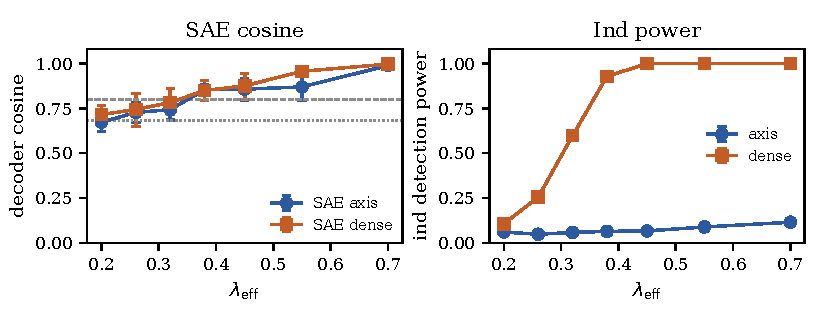
\includegraphics[width=\linewidth,height=1.45in,keepaspectratio]{figures/fig_sae_wall.pdf}
\caption{\textbf{Strength sweep.} (a) TopK cosine rises with $\lambda_{\mathrm{eff}}$ for both geometries; (b) independence power retains the axis--dense gap. Dotted: chance; dashed: frozen $0.80$.}
\label{fig:wall}
\vspace{-0.5em}
\end{figure}

\subsection{Training-only spectral structure improves matched-compute recovery}
We test a practical intervention: initialize a signed decoder pair from the training covariance, then train the otherwise unconstrained SAE. The paired $3$-objective $\times$ $2$-capacity $\times$ $2$-geometry $\times$ $4$-seed matrix shares data and all seeds; only initialization differs. Target and validation data are withheld from training and readout selection.

\begin{figure}[ht]
\centering
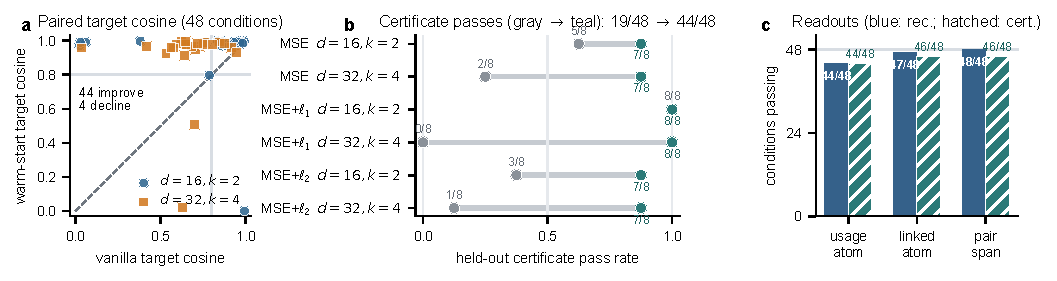
\includegraphics[width=\linewidth,height=1.20in,keepaspectratio]{figure3_bestpaper/output/figure3_spectral_warm_start.pdf}
\caption{\textbf{Training-only spectral warm start.} Paired target cosines, held-out certificate passes, and three selection-blind readouts under matched compute. Gray: vanilla; teal: warm. Only initialization differs.}
\label{fig:warmstart}
\vspace{-0.5em}
\end{figure}

Warm start raises recovery from $23/48$ to $44/48$ and certificate passes from $19/48$ to $44/48$; cosine improves in $44/48$ pairs (mean $+0.199$). The independent eight-seed replication gives $39/96$ versus $89/96$ recovery and $35/96$ versus $88/96$ certification, with cluster gains $0.521$ (bootstrap $95\%$ CI $[0.417,0.625]$) and $0.232$ ($[0.151,0.308]$). No post-initialization constraint is imposed, so this is not an all-condition claim.

\iffalse
\begin{figure}[H]
\centering
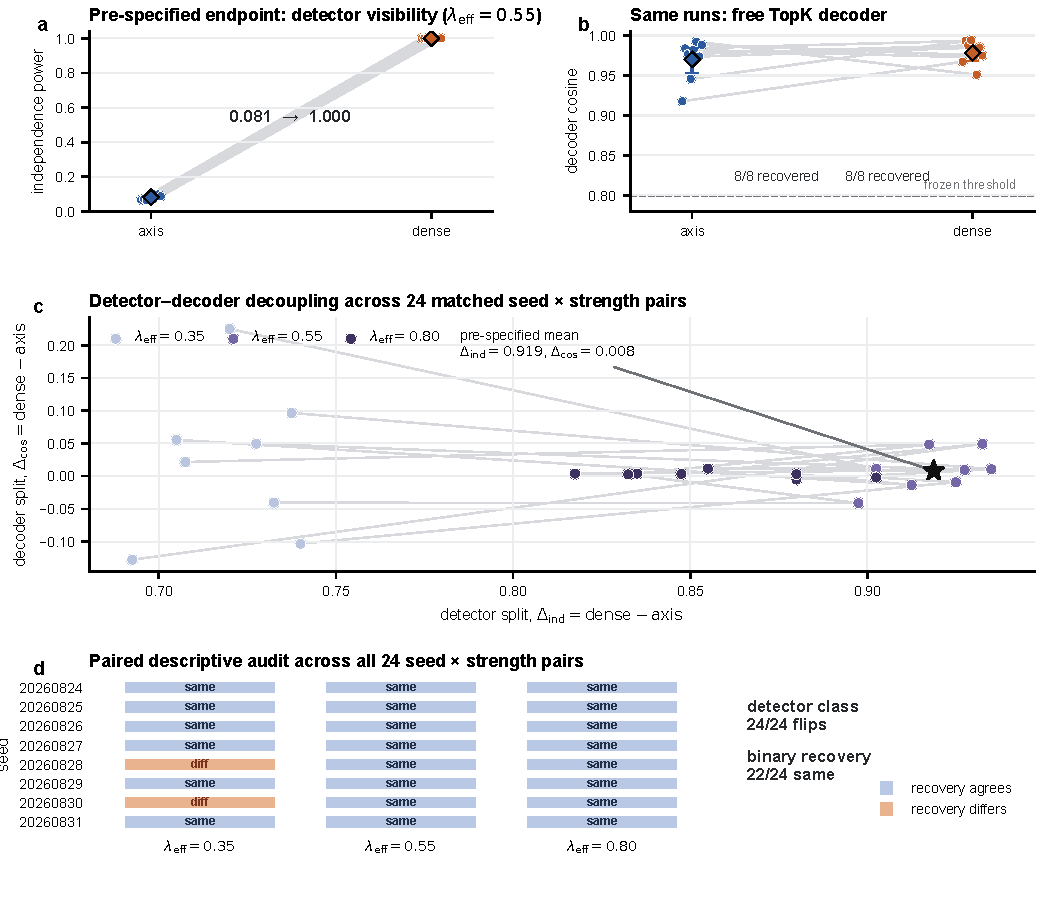
\includegraphics[width=\linewidth]{figures/fig2_detector_decoder.pdf}
\caption{\textbf{Detector--decoder decoupling in the matched E4-v2 control.}
\textbf{(a)} At the primary endpoint $\lambda_{\mathrm{eff}}=0.55$, the fixed-basis independence detector splits axis and dense loadings, while label and covariance power are matched.
\textbf{(b)} The same TopK protocol recovers both geometries in all eight seeds at the frozen recovery threshold $0.80$.
\textbf{(c)} Across all $24$ matched seed--strength pairs, independence power changes sharply with geometry but decoder cosine remains close to the identity; the diamond is the mean paired difference, not a seed observation.
\textbf{(d)} Detector-class flips occur in $24/24$ pairs, while recovery agrees in $22/24$.
Points and connecting lines are the observed paired records; intervals in panels (a,b) are seed-level bootstrap $95\%$ confidence intervals from $1000$ percentile resamples.
Panel (d) is a paired descriptive audit, not a second pre-specified endpoint.}
\label{fig:sae_control}
\end{figure}
\fi

\iffalse
Figure~\ref{fig:exp} tests Theorem~\ref{thm:recon} at chance $\approx 0.36$, cosine $0.80$. Gray curves are first-principles rates. Labels track $\lambda^{-2}$ ($-1.96$/$-1.99$). Empirical PCA slopes are $-4.09$/$-3.66$. Rank-1 linear GD does not inherit $C{=}0$ ($-2.60$/$-3.09$) but crosses $0.80$ later than PCA: the trained linear exponent is not the closed-form one. A $1$-atom $z$-clamp still sits at $2.7$--$3.5\mathrm{k}$ on the axis, the same floor as the $16$-atom oracle. Free TopK sits above PCA ($-2.97$/$-4.33$). No $C{=}0$ hole.

\begin{figure}[H]
\centering
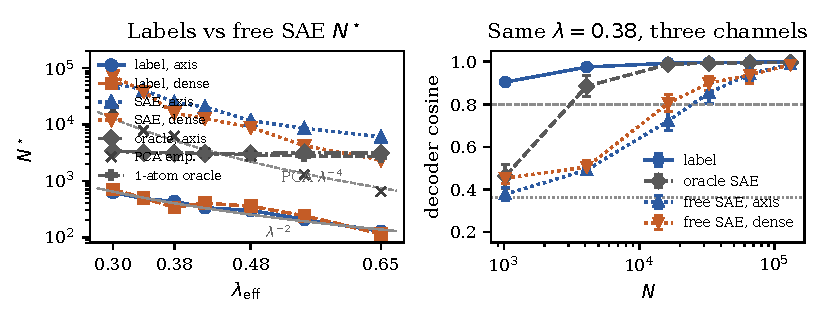
\includegraphics[width=\linewidth]{figures/fig_sae_exponent.pdf}
\caption{\textbf{Left:} constant-epoch $N^\star(\lambda)$ in $m=32$, shared cosine $0.80$, same seven $\lambda$. Gray: conditional-isolation $\lambda^{-2}$ and PCA $\lambda^{-4}$ benchmarks. Crosses: empirical PCA. \textbf{Right:} cosine versus $N$ at $\lambda_{\mathrm{eff}}=0.38$. Oracle clamps $z$ into atom $0$. Dotted: chance. Dashed: $0.80$.}
\label{fig:exp}
\end{figure}

Figure~\ref{fig:floor} visualizes the same residual-floor controls. To connect Proposition~\ref{prop:rom} to a \emph{trained} decoder, we use an $80$-feature mixture ($8$ axis-aligned, $72$ random) with heavy-tailed $\lambda$. Under Protocol A (dictionary $192$, $k=8$), mean recovery is $0.91$ for axis features and $0.85$ for random directions; axis features account for only $6\%$ of misses. Protocol B fixes $N=16384$, $k=4$, and varies dictionary size: missed-variance share falls from $0.79$ at $d=8$ to $0.06$ at $d=256$, while the independence predictor remains near $0.11$. The quartic detectability prediction is nearly zero at this $N$ and is only a lower bound. Its correlation with missed mass is $0.013$, so the excess floor may reflect capacity, absorption, optimization, correlation, or nonlinearity rather than an axis rule.

\begin{figure}[H]
\centering
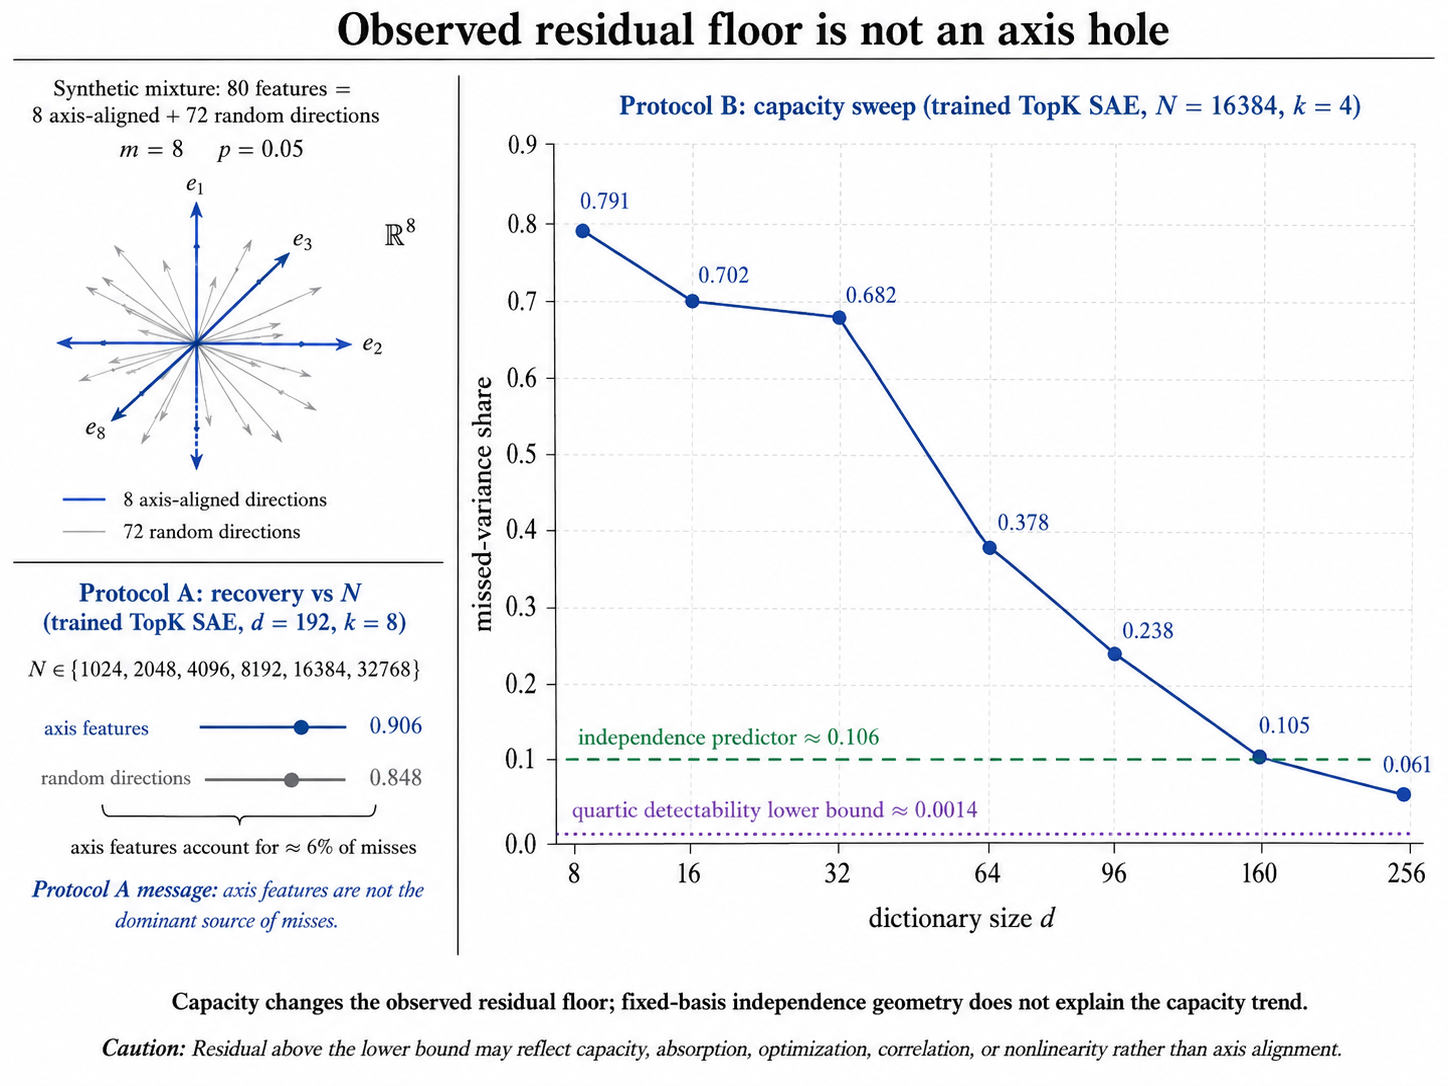
\includegraphics[width=\linewidth]{figures/figA_residual_floor.png}
\caption{Residual-floor controls on the same known $80$-feature mixture. Protocol A compares recovery by geometry at dictionary $192$, $k=8$; Protocol B varies dictionary size at $N=16384$, $k=4$. Capacity changes the observed floor, whereas the fixed-basis independence predictor does not track the sweep. The quartic curve is a detectability lower bound, not a trained-SAE identity.}
\label{fig:floor}
\end{figure}
\fi

\subsection{Real residuals transfer the detector hole and warm-start gain}
\label{sec:gpt2}
On GPT-2-small layer-$6$ and Pythia-70m layer-$3$ residuals from a SHA-recorded WikiText-2 file, we fit train-split PCA whitening and inject Bernoulli features along $e_1$, $e_{32}$, and a dense loading. The eight-seed matched TopK matrix ($d=64,k=4$; cosine $\ge0.80$) changes only random versus training-spectral initialization at strengths $0.35$ and $0.55$.

\begin{figure}[ht]
\centering
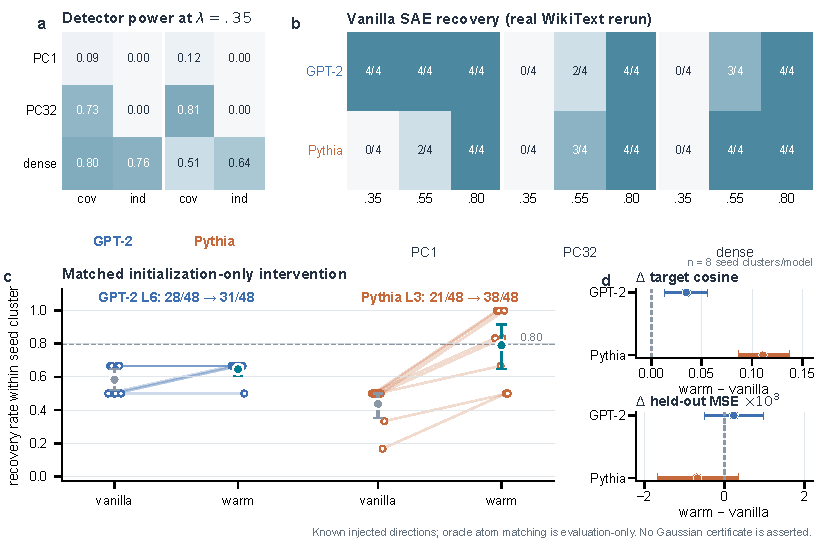
\includegraphics[width=\linewidth,height=2.05in,keepaspectratio]{figure4_lm_validation/output/figure_lm_validation.pdf}
\caption{\textbf{Transfer to empirical residuals.} Known-direction detector power, vanilla recovery counts, paired cluster recovery, and warm-minus-vanilla effects on real WikiText residuals. Oracle matching is evaluation-only; no Gaussian certificate is asserted.}
\label{fig:gpt2}
\vspace{-0.6em}
\end{figure}

Figure~\ref{fig:gpt2} transfers both the split and the frozen-budget intervention. At $\lambda=0.35$, independence power is $0$ on both PCA axes but $0.764/0.640$ on the dense loading; covariance is low only on PC1. Recovery changes from $28/48$ to $31/48$ for GPT-2 and $21/48$ to $38/48$ for Pythia, with cosine gains $0.035$ ($95\%$ CI $[0.013,0.056]$) and $0.111$ ($[0.086,0.137]$); both MSE intervals include zero. The Pythia-160M extension changes recovery from $28/48$ to $33/48$ and cosine by $+0.034$ ($95\%$ CI $[0.018,0.049]$), but increases MSE by $0.000665$ ($95\%$ CI $[0.000389,0.000980]$). The gain is model- and budget-dependent; details are in Appendix~\ref{app:gpt2}.

\iffalse
\begin{figure}[H]
\centering
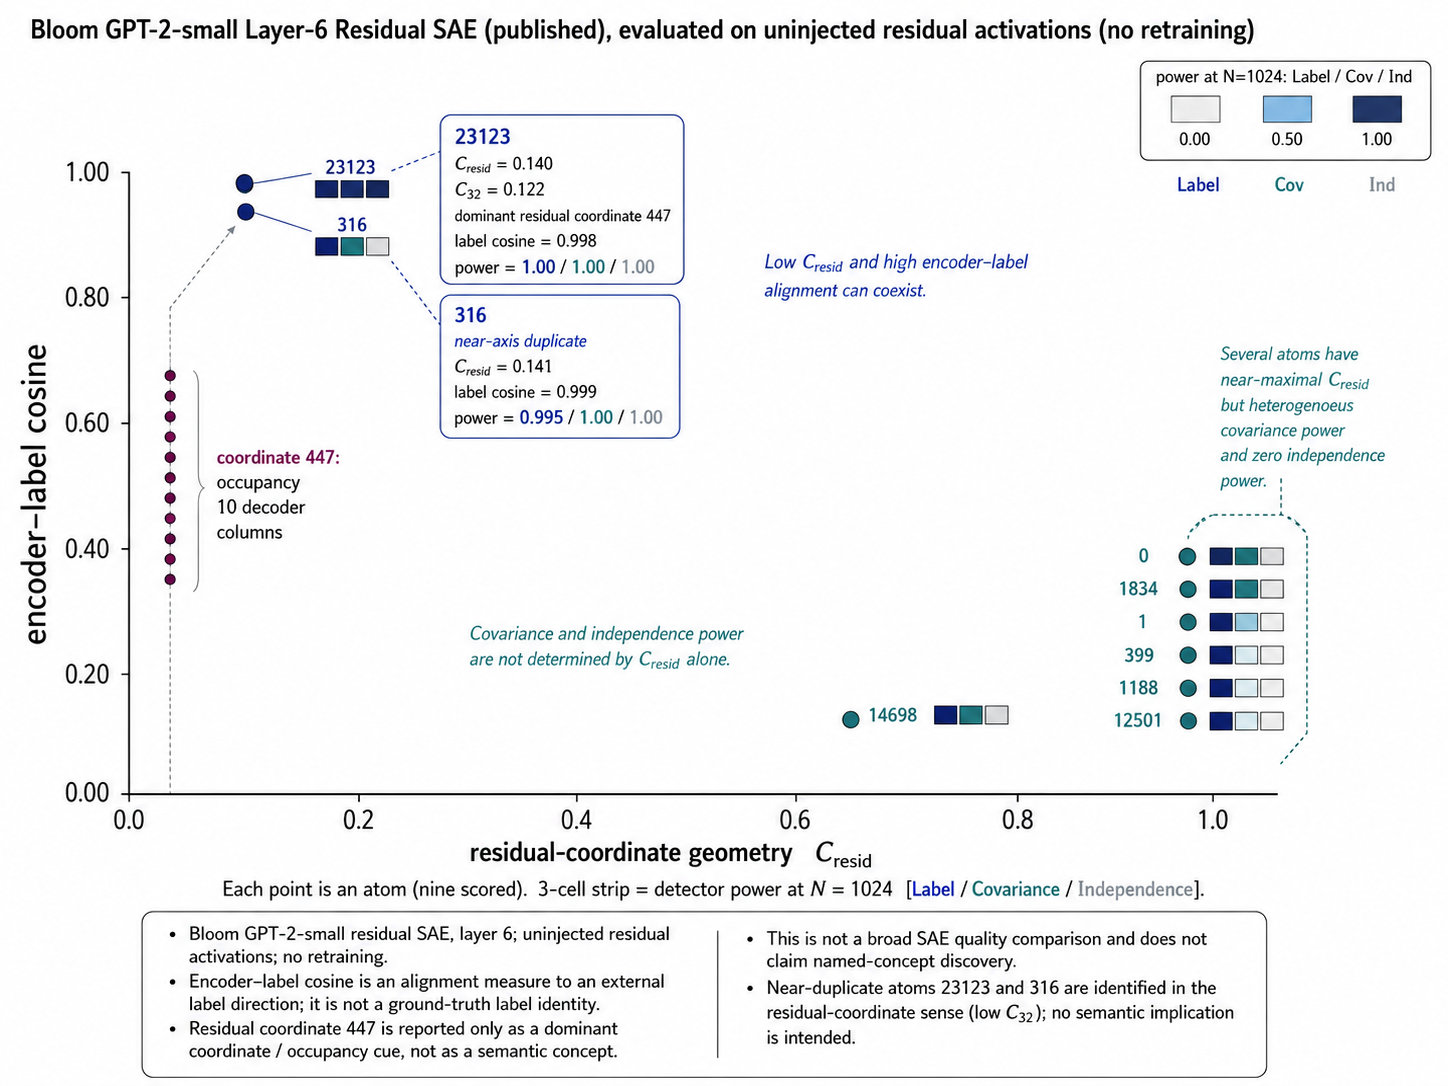
\includegraphics[width=\linewidth]{figures/figA_public_atoms.png}
\caption{Published Bloom GPT-2-small layer-$6$ residual SAE, evaluated without injection or retraining. Nine scored atoms show that low residual-coordinate $C$ can coexist with high encoder-label alignment; detector power at $N=1024$ is not determined by $C$ alone. Labels denote specified external directions, not discovered concepts.}
\label{fig:public_atoms}
\end{figure}

\vspace{-0.4em}
\begin{table}[H]
\caption{Four representative Bloom layer-$6$ atoms; complete nine-atom geometry, alignment, and $N=1024$ power scores are in the JSON artifact. Lab cos. is encoder-label cosine to a specified external direction, not a concept-discovery score.}
\label{tab:diag}
\begin{center}
\footnotesize
\setlength{\tabcolsep}{4pt}
\begin{tabular}{@{}rrrlc@{}}
\toprule
\textbf{Atom} & $\boldsymbol{C}$ & $\boldsymbol{C_{32}}$ & \textbf{Documented as} & \textbf{Lab cos.} \\
\midrule
$23123$ & $0.140$ & $0.122$ & residual $447$ ($\times 10$) & $1.00$ \\
$1$ & $0.996$ & $0.862$ & grants / funding & $1.00$ \\
$1834$ & $0.996$ & $0.904$ & {VAT} / tax terms & $0.995$ \\
$0$ & $0.996$ & $0.902$ & notice / realization & $1.00$ \\
\bottomrule
\end{tabular}
\end{center}
\end{table}
\fi

\section{Discussion}
\label{sec:disc}
\iffalse
The axis hole is real, but it belongs to a fixed-basis independence test rather than to unconstrained sparse decoders. For a stronger but explicitly structured family, Theorem~\ref{thm:spectral_anchor} proves objective/capacity-uniform recovery: all residual objectives inherit a target-free signed spectral anchor when the anchor-preserving constraints and finite-sample eigengap condition hold. The matched E4-v2 control makes the boundary explicit: at fixed strength, independence power differs by $0.919$ (axis $0.081$ versus dense $1.000$), while the same free TopK protocol recovers both geometries in all eight seeds. Across the full three-strength grid, the cov-not-ind class and the visible class each recover $19/24$ configurations. The paired descriptive check flips detector class in all $24/24$ seed-strength pairs, while recovery agrees in $22/24$; this is not an additional pre-specified endpoint. This is a controlled non-implication, not a universal statement about training. The objective-agnostic reconstruction certificate (Theorem~\ref{thm:certificate}) supplies the complementary guarantee: after any objective has produced a frozen decoder subspace, an independent held-out risk comparison yields the same target-alignment bound regardless of how that subspace was obtained. It certifies outputs, not optimization convergence. Free-SAE misses can still reflect strength, sample size, capacity, absorption, optimization, correlation, or nonlinearity; PCA-axis alignment alone does not explain them. Linear reconstruction is quartic, whereas a conditional isolation stage is quadratic once a separator is available, and neither rate contains a $C{=}0$ axis term. Atom $23123$ is near-axis in the residual-coordinate frame and strongly aligned with its encoder-label direction. The published SAE allocates atoms to that direction; this specified-direction result does not imply named-concept discovery.

\paragraph{Limitations.}
The GPT-2/Pythia transfer is known-direction injection; uninjected token recovery and published-atom scores are specified-direction, not named concepts. The PC1 covariance split is leftover structure, not the independence hole. Proposition~\ref{prop:rom} is a lower bound; TopK $N^\star$ is nonconvex and sits above PCA. The E4-v2 non-implication is limited to this three-strength, eight-seed TopK control and does not establish recovery equivalence for other SAE objectives, widths, or unknown-direction discovery. An independent held-out capacity/sparsity grid is reported in Appendix~\ref{app:confirm}: its composite gate fails at $d{=}32,k{=}4$ because dense recovery is $0.625<0.75$, so it does not broaden the E4-v2 claim. A subsequent post-hoc same-trajectory budget trace reaches dense recovery $0.875$ at $16$k steps, supporting a training-budget explanation without revising the original confirmation decision. The new spectral-anchor experiments are separate structured constructions: the exact-anchor v3 family passes all $48/48$ rows, and the relaxed bounded-drift v4 family also passes all $48/48$ rows with a trainable anchor, maximum drift $0.1287$ radians, nonzero residual leakage capped at $0.10$, and a certified cosine lower bound of $0.8543$. The v4 result relaxes the hard v3 constraints but still uses an explicit trust-region/data--target linkage; neither result implies recovery for unconstrained SAEs. A separate $72$-row dose-response control (Appendix~\ref{app:exp}) shows that recovery of the spectral direction is mechanism-independent at this scale---the unconstrained control also recovers all eight anchor groups---but it converges to degenerate high-leakage dictionaries, with a residual--anchor dot product up to $0.734$ and the worst held-out reconstruction loss (mean loss contrast not significant at $n{=}8$; the robust gaps are leakage and variance); the certified family therefore buys provable leakage control and lower variance, not recovery itself.

\fi

The independence-detector axis blind spot need not transfer to free TopK recovery. A held-out certificate validates a frozen decoder subspace, not optimization; spectral initialization improves recovery/alignment but can trade against reconstruction cost. The anchor-preserving theorem is stronger only under its stated constraints.

\paragraph{Limitations.}
Evidence remains bounded to controlled synthetic features and known injections in GPT-2/Pythia models; observed failures rule out all-condition, unconstrained-training, or unknown-semantic guarantees.

{\footnotesize
\bibliography{refs}
\bibliographystyle{iclr2027_conference}
}

\section*{Use of AI tools}
Generative AI tools were used to implement experiment scripts, to assist with \LaTeX{} drafting, and to help organize proofs already derived in the technical appendix. They were not used to formulate the mathematical claims or as a source of those claims. The authors take responsibility for the theorems, experiments, and remaining errors.

\appendix
{\footnotesize
\section{Additional empirical details}
\label{app:additional}
This appendix records secondary diagnostics that are useful for auditing the claim boundary but are not needed for the main detector--decoder comparison.

\subsection{Residual-floor derivation}
\label{app:additional_floor}
Let $\beta_N$ be the decision threshold induced by the model-selection rule. For $C_i>0$, define
\begin{equation}
\lambda_{c,i}(N)=\Bigl(\frac{\beta_N}{N C_i}\Bigr)^{1/4},\qquad
f_{\mathrm{dark}}(N)=\frac{\sum_i \lambda_i^2\,1\{\lambda_i<\lambda_{c,i}(N)\}}{\sum_i \lambda_i^2}.
\end{equation}
If $C_i=0$, set $\lambda_{c,i}(N)=\infty$ for that detector class. For unconstrained reconstruction, Theorem~\ref{thm:recon} replaces $C_i$ by a positive constant for the linear encoder and gives a conditional $\lambda^{-2}$ isolation benchmark after a separating direction is available.

\begin{theorem}[Critical boundary and dark-matter fraction]
\label{thm:floor}
Under Theorem~\ref{thm:quartic}, the subcritical set at sample size $N$ is $I_{\mathrm{dark}}(N)=\{i:\lambda_i<\lambda_{c,i}(N)\}$, and $f_{\mathrm{dark}}(N)$ is the variance share of that set. If $\beta_N\asymp\log N$ and $\Pr(\lambda\le x)\asymp x^{\alpha}$ near zero, then $f_{\mathrm{dark}}(N)\asymp(\log N/N)^{(\alpha+2)/4}$.
\end{theorem}

\begin{proposition}[Recover-or-miss residual identity]
\label{prop:rom}
Under the recover-or-miss idealization that supercritical features contribute negligible residual variance and subcritical features contribute their full variance, the irreducible feature-level reconstruction floor equals $f_{\mathrm{dark}}(N)$.
\end{proposition}

Proposition~\ref{prop:rom} is an idealization, not a trained-SAE identity. It supplies a detectability lower bound: optimization failure, absorption, correlated latents, and nonlinear features can add residual error above this floor.

\begin{table}[H]
\caption{Synthetic suite. Intervals are seed-level bootstrap $95\%$ confidence intervals. These rows summarize secondary controls; the matched E4-v2 endpoint remains in the main text.}
\label{tab:results}
\begin{center}
\scriptsize
\begin{tabular}{@{}>{\raggedright\arraybackslash}p{0.36\linewidth}>{\raggedright\arraybackslash}p{0.56\linewidth}@{}}
\toprule
\textbf{Check} & \textbf{Result} \\
\midrule
Detector $N^\star(\lambda)$ slope & $-1.95$ vs. $-3.72$ (theory: $-2$ vs. $-4$) \\
Same-$\lambda$ independence power & axis $0.096$ $[0.090,0.102]$; dense $0.969$ $[0.965,0.974]$ \\
Rotate $B$, hold $\lambda$ & ind vs. $1-\lVert B^\top w\rVert_4^4$: $r=0.977$; label $\equiv 1$ \\
2-sparse imbalance $\varepsilon$ & $0.123$ ($\varepsilon{=}0.01$) $\to$ $0.810$ ($\varepsilon{=}0.50$) \\
Ind recover-or-miss floor & predicted vs. missed variance $r=0.999$, MAE $0.005$ \\
TopK cosine vs. $\lambda$ & axis/dense $0.85/0.85$ at $0.38$; $0.32$ remains near chance \\
Label vs. SAE $N^\star$ ($m{=}32$) & $-1.96/-1.99$ vs. $-2.97/-4.33$ (Theorem~\ref{thm:recon}) \\
\bottomrule
\end{tabular}
\end{center}
\end{table}

\subsection{Strength sweep}
The full strength sweep shows that TopK recovery remains strength-dependent in both geometries.
\begin{figure}[H]
\centering
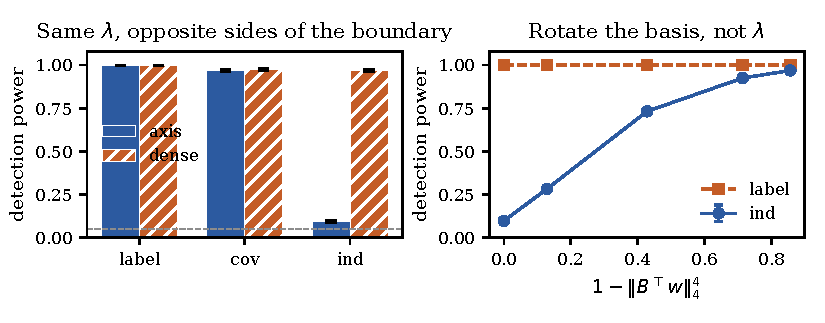
\includegraphics[width=\linewidth]{figures/fig_same_lambda.pdf}
\caption{Matched-strength detector calibration. Left: only the feature-independent statistic shows the axis--dense geometry gap. Right: rotating the detector basis at fixed signal strength moves independence power while label power remains one.}
\label{fig:same_appendix}
\end{figure}

\begin{figure}[H]
\centering
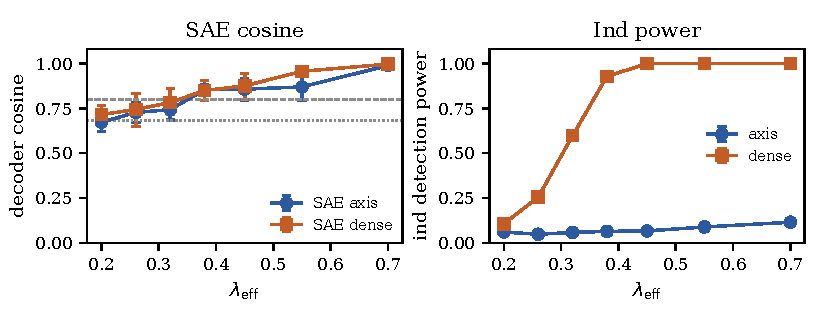
\includegraphics[width=\linewidth]{figures/fig_sae_wall.pdf}
\caption{Strength sweep for the free TopK decoder and fixed-basis independence detector. Recovery rises with signal strength in both geometries, while independence power retains an axis--dense gap.}
\label{fig:wall_appendix}
\end{figure}

\subsection{Reconstruction-rate and residual-floor diagnostics}
\label{app:secondary}
The reconstruction-rate controls test Theorem~\ref{thm:recon} at chance $\approx 0.36$ and cosine $0.80$. Labels track $\lambda^{-2}$, empirical PCA tracks approximately $\lambda^{-4}$, and trained linear or TopK encoders do not acquire a $C{=}0$ axis hole. The residual-floor controls use an $80$-feature mixture ($8$ axis-aligned, $72$ random) with heavy-tailed strengths. At dictionary $192$, $k=8$, mean recovery is $0.91$ for axis features and $0.85$ for random directions; axis features account for only $6\%$ of misses. At fixed $N=16384$, $k=4$, missed-variance share falls from $0.79$ at $d=8$ to $0.06$ at $d=256$, while the independence predictor remains near $0.11$; its correlation with missed mass is $0.013$.

\begin{figure}[H]
\centering
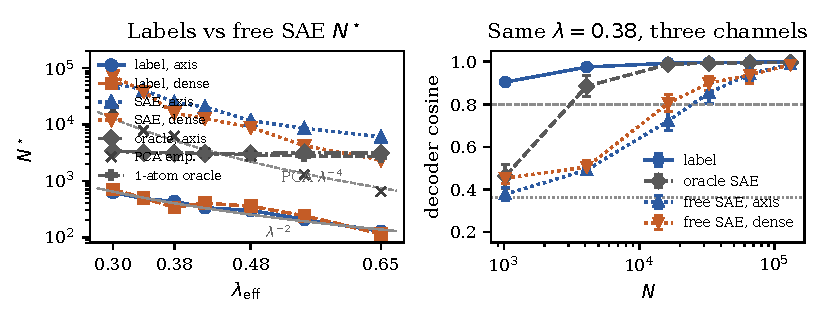
\includegraphics[width=\linewidth]{figures/fig_sae_exponent.pdf}
\caption{Constant-epoch $N^\star(\lambda)$ and cosine-versus-$N$ controls in $m=32$ at shared cosine threshold $0.80$. Gray curves are conditional-isolation and PCA benchmarks; the empirical and trained encoders do not show an axis-specific $C{=}0$ floor.}
\label{fig:exp}
\end{figure}

\begin{figure}[H]
\centering
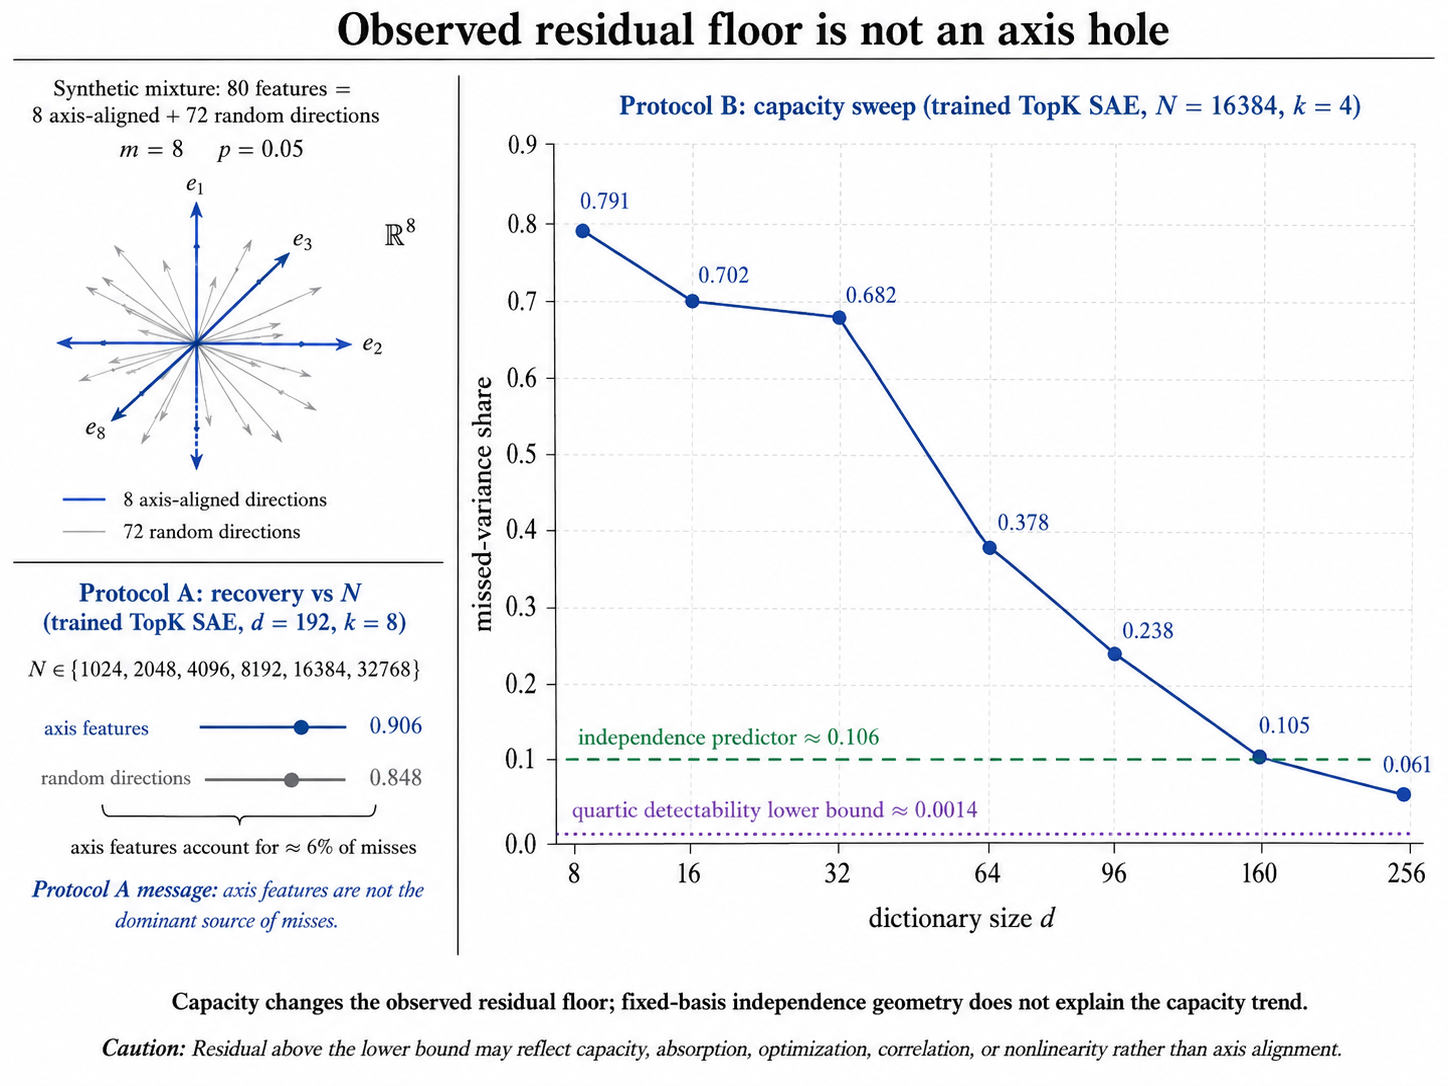
\includegraphics[width=\linewidth]{figures/figA_residual_floor.png}
\caption{Residual-floor controls on the known $80$-feature mixture. Capacity changes the observed floor, whereas the fixed-basis independence predictor does not track the sweep. The quartic curve is a detectability lower bound, not a trained-SAE identity.}
\label{fig:floor}
\end{figure}

\subsection{GPT-2/Pythia residual transfer and public atoms}
\label{app:gpt2}
The corrected bridge uses an explicit real WikiText-2 file, with no synthetic-text fallback, and fits PCA whitening on the training split. GPT-2-small layer-$6$ and Pythia-70m layer-$3$ receive Bernoulli injections along two whitened axes and a dense loading. The independence detector fails on both tested axes, whereas fixed-background covariance fails only on PC1. The main text reports the separate eight-seed matched warm-start intervention; the Pythia-160M layer-$6$ scale extension and its budget follow-up are reported below. Without injection, TopK recovery of token difference-of-means directions and the public-SAE atom audit remain specified-direction diagnostics rather than named-concept discovery.

\begin{figure}[H]
\centering
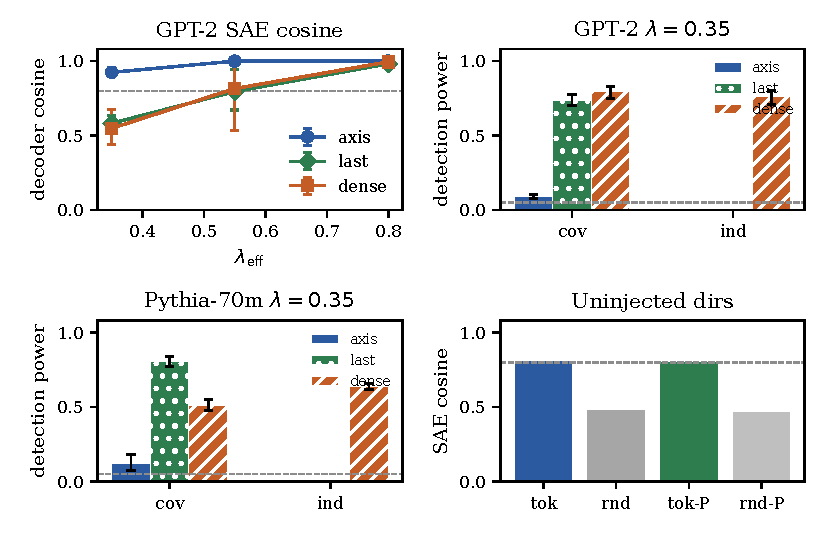
\includegraphics[width=\linewidth,height=2.55in,keepaspectratio]{figures/fig_gpt2.pdf}
\caption{Corrected real-WikiText GPT-2/Pythia residual bridge. Top: injected-feature cosine and detector controls. Bottom: the Pythia repeat and uninjected token-direction recovery. Labels denote known injected or externally specified directions, not discovered concepts.}
\label{fig:gpt2_appendix}
\end{figure}

A published GPT-2 residual SAE~\citep{bloom2024gpt2sae} with $24{,}576$ atoms has minimum residual-coordinate $C=0.140$; ten near-duplicate columns concentrated on residual coordinate $447$ comprise the $0.04\%$ below $0.20$. This is an evaluation of a published decoder without retraining and does not establish named-concept discovery.

\begin{figure}[H]
\centering
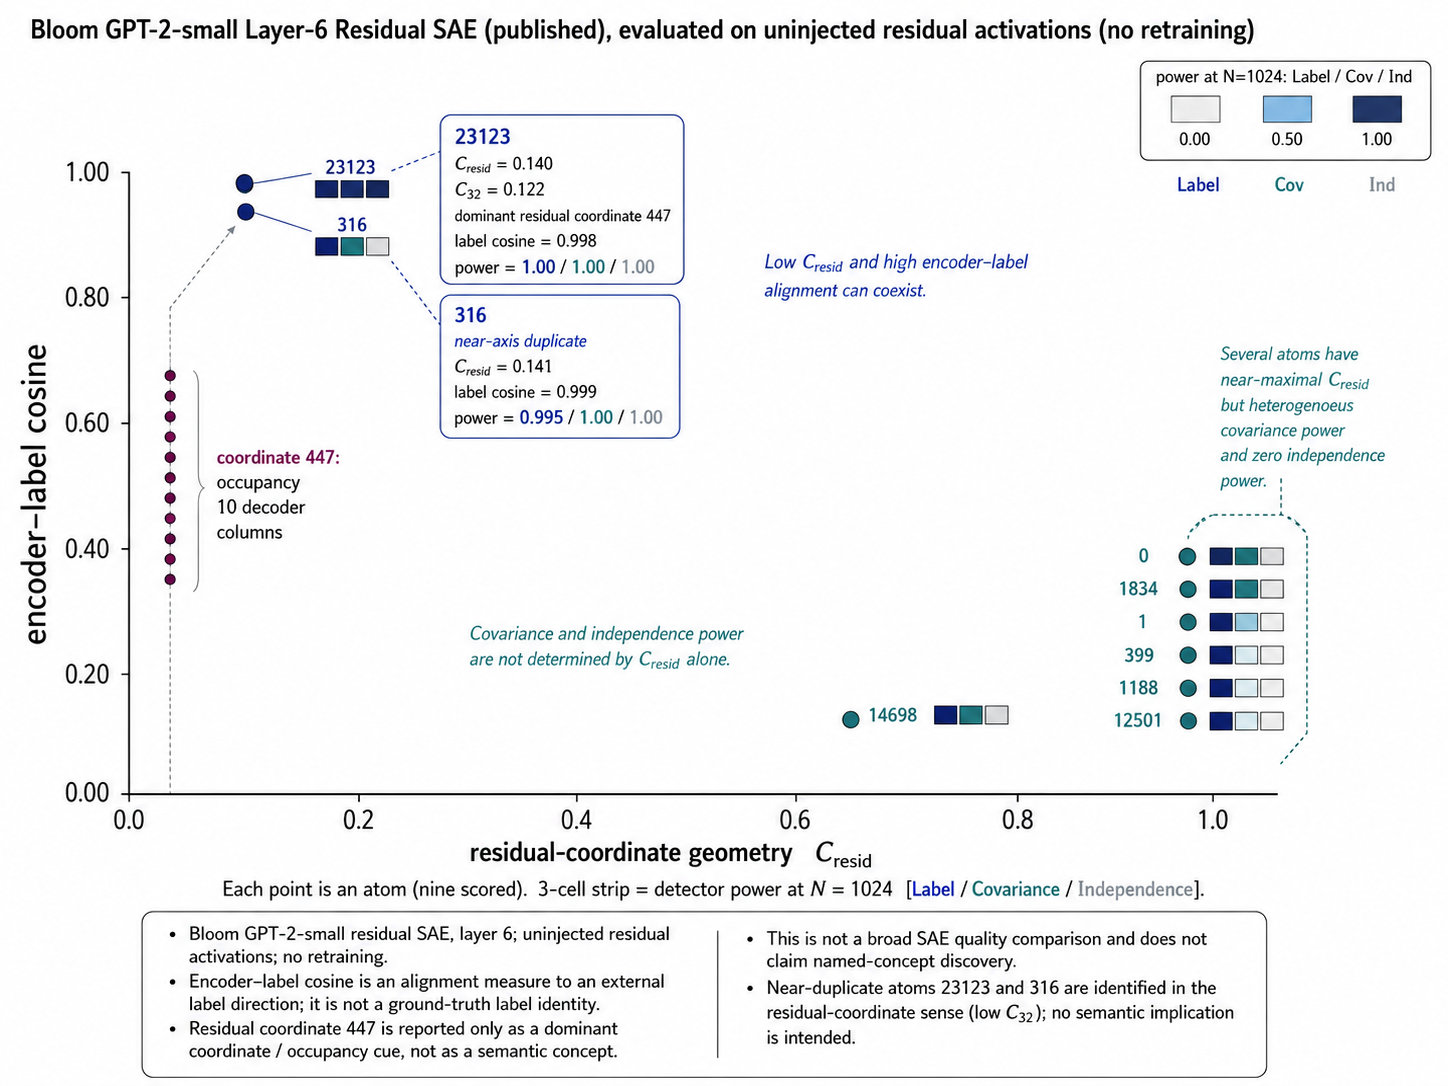
\includegraphics[width=\linewidth]{figures/figA_public_atoms.png}
\caption{Published Bloom GPT-2-small layer-$6$ residual SAE evaluated without injection or retraining. Low residual-coordinate $C$ can coexist with high alignment to a specified external direction.}
\label{fig:public_atoms}
\end{figure}

\begin{table}[H]
\caption{Representative Bloom layer-$6$ atoms. Lab cos. is alignment to a specified external direction, not a concept-discovery score.}
\label{tab:diag}
\begin{center}
\scriptsize
\setlength{\tabcolsep}{4pt}
\begin{tabular}{@{}rrrlc@{}}
\toprule
\textbf{Atom} & $\boldsymbol{C}$ & $\boldsymbol{C_{32}}$ & \textbf{Documented as} & \textbf{Lab cos.} \\
\midrule
$23123$ & $0.140$ & $0.122$ & residual $447$ ($\times 10$) & $1.00$ \\
$1$ & $0.996$ & $0.862$ & grants / funding & $1.00$ \\
$1834$ & $0.996$ & $0.904$ & {VAT} / tax terms & $0.995$ \\
$0$ & $0.996$ & $0.902$ & notice / realization & $1.00$ \\
\bottomrule
\end{tabular}
\end{center}
\end{table}

\section{Proofs}
\label{app:proofs}

\subsection{Gaussian identities}
\label{app:gauss}
\begin{lemma}
\label{lem:kl}
If $P=\mathcal{N}(0,\Sigma_1)$ and $Q=\mathcal{N}(0,\Sigma_0)$ are nondegenerate,
$D_{\mathrm{KL}}(P\Vert Q)=\tfrac12\bigl(\mathrm{tr}(\Sigma_0^{-1}\Sigma_1)-m+\log\det\Sigma_0-\log\det\Sigma_1\bigr)$.
\end{lemma}
\begin{lemma}
\label{lem:det}
For $s>0$, $\lambda\ge 0$, and $\lVert w\rVert=1$, $\det(s^2 I_m+\lambda^2 ww^{\top})=s^{2m}(1+\lambda^2/s^2)$.
\end{lemma}

\subsection{Labeled quadratic benchmark}
Assume the activation indicator $z_i$ is observed and $h=z_i W_i+u$ with $u\sim\mathcal{N}(0,\sigeff^2 I_m)$. Then $D_{\mathrm{KL}}(\mathcal{N}(W_i,\sigeff^2 I)\Vert\mathcal{N}(0,\sigeff^2 I))=\lVert W_i\rVert^2/(2\sigeff^2)$. The expected information per observation is of order $\lambda_i^2$, so $N_i^*\asymp\sigeff^2\lambda_i^{-2}$.

\subsection{Proof of Theorem~\ref{thm:quartic}}
\label{app:thm2}
Let $\Sigma_1=s^2 I+\lambda^2 ww^{\top}$ and $D(d)=\mathrm{diag}(d)$. The KL $\Phi(d)=\tfrac12\sum_j\bigl((\Sigma_1)_{jj}/d_j+\log d_j\bigr)+\mathrm{const}$ decouples. The unique minimizer is $d_j^\star=(\Sigma_1)_{jj}=s^2+\lambda^2 w_j^2$. Substituting yields $\mathrm{tr}(D_\star^{-1}\Sigma_1)=m$, so
\begin{equation}
D_{\mathrm{loc}}(\lambda)=\tfrac12\Bigl(\sum_{j=1}^m\log(1+t w_j^2)-\log(1+t)\Bigr),\qquad t=\lambda^2/s^2.
\end{equation}
The expansion $\log(1+u)=u-u^2/2+O(u^3)$ and $\sum_j w_j^2=1$ give
$\sum_j\log(1+t w_j^2)-\log(1+t)=\tfrac{t^2}{2}(1-\lVert w\rVert_4^4)+O(t^3)$.
Multiplying by $1/2$ produces $D_{\mathrm{loc}}=C\lambda^4+O(\lambda^6)$ with $C=(1-\lVert w\rVert_4^4)/(4s^4)$. Accumulated evidence $N D_{\mathrm{loc}}$ must stay bounded away from zero, hence $N^*\asymp C^{-1}\lambda^{-4}$. If $w=e_j$ the exact KL is identically zero.

\subsection{Projection identity}
\label{app:proj}
Write the local perturbation parameter as $\eta=\lambda^2$. The log-likelihood of $P_\eta$ against $P_0$ has score $\psi_w$. A regular local parameterization of $\mathcal{M}$ has scores in $T$. The second-order local KL is the least-squares residual $\eta^2/2\,\lVert\psi_w-\Pi_T\psi_w\rVert^2+O(\eta^3)$. Substituting $\eta=\lambda^2$ yields Proposition~\ref{prop:proj}. For the diagonal family, $T$ is spanned by $e_j(h)=(h_j^2-s^2)/(2s^4)$. Then $\Pi_T\psi_w=\sum_j w_j^2 e_j$ and the residual is $(2s^4)^{-1}\sum_{j\neq\ell}w_j w_\ell h_j h_\ell$, with $L^2$ norm squared $(1-\lVert w\rVert_4^4)/(2s^4)$, recovering Theorem~\ref{thm:quartic}.

\subsection{Proof of Theorem~\ref{thm:saeclass}}
Take $D$ with first column $w$ and remaining columns arbitrary unit vectors, and $z=\alpha e_1$. Then $Dz=\alpha w$ for every unit $w$, including $w=e_j$. The rank-one mean-shift family is therefore in the closure of $\mathcal{F}_k$, including at $C_{\mathrm{ind}}=0$. This establishes availability of the axis direction; it makes no claim about the optimization path or about projecting probability models onto $\mathcal{F}_k$. By contrast, $\Mind$ contains every diagonal spike, which is why $C_{\mathrm{ind}}=0$ at $w=e_j$.

\subsection{Proof of Proposition~\ref{prop:unconstrained_no_bound}}
Fix a unit target $w$ and choose any unit $v\perp w$, which exists because $m\ge2$. Let the first decoder column be $v$ and choose a one-sparse code $z=\alpha e_1$. Then $Dz=\alpha v$ is feasible in $\mathcal{F}_k$, but its alignment with $w$ is $|v^\top w|=0$. Since the construction is feasible for every target and the class contains both aligned and orthogonal choices, membership in $\mathcal{F}_k$ cannot imply a positive target-uniform alignment lower bound. The argument quantifies over feasible decoders only; it does not describe a learner that observes samples and selects $v$.

\subsection{Proof of Theorem~\ref{thm:certificate}}
For any orthogonal projector $P$, $R(P)=\mathrm{tr}((I-P)\Sigma)$. Since $P_w$ has rank $r$ and contains $w$, $\mathrm{tr}(P_w\Sigma)=r\sigma^2+\tau$. For $P$, $\mathrm{tr}(P\Sigma)=r\sigma^2+\tau w^{\top}Pw$, so subtraction gives $R(P)-R(P_w)=\tau(1-w^{\top}Pw)=\tau(1-\lVert Pw\rVert^2)$.

For the validation statement, the difference of the two projected quadratic losses is a centered Gaussian quadratic form after subtracting its expectation. The standard Gaussian quadratic-form tail bound for the difference of two rank-$r$ projectors (whose difference has rank at most $2r$) gives, with probability at least $1-\delta$, an error at most $2(\sigma^2+\tau)(\sqrt{4r\log(2/\delta)/n}+\log(2/\delta)/n)$. Substituting this upper confidence bound for the excess risk into the exact identity yields the stated cosine lower bound. The proof uses only the frozen projector and the held-out samples; it does not use how the projector was produced.

\subsection{Proof of Theorem~\ref{thm:spectral_anchor}}
For the population covariance, $w$ is the simple leading eigenvector and the eigengap is $\tau$. The standard eigenvector perturbation bound for a symmetric perturbation $E=S-\Sigma$ gives $\sin\angle(\widehat u,w)\le \lVert E\rVert_{\mathrm{op}}/(\tau-\lVert E\rVert_{\mathrm{op}})$ whenever $\lVert E\rVert_{\mathrm{op}}<\tau/2$. A Gaussian sample-second-moment bound follows by applying the extreme singular-value inequality to $\Sigma^{-1/2}[X_1,\ldots,X_N]$: with probability at least $1-\delta'$, $\lVert S-\Sigma\rVert_{\mathrm{op}}\le \lVert\Sigma\rVert_{\mathrm{op}}(2q+q^2)$ for $q=(\sqrt m+\sqrt{2\log(2/\delta')})/\sqrt N$. A union bound over the $G$ training anchors uses $\delta'=\delta/G$. The signed pair is implemented by nonnegative anchor activations, so it uses one active feature slot; projecting each residual decoder column onto $\widehat u^\perp$ makes residual updates unable to change the anchor component. Hence residual objective, optimizer, initialization, and residual capacity do not enter the anchor direction or its bound.

\subsection{Proof of Theorem~\ref{thm:bounded_drift_anchor}}
Let $\theta_0=\angle(\widehat u_0,w)$ and $\theta=\angle(\widehat u,w)$. The spherical triangle inequality gives $\theta\le\theta_0+\angle(\widehat u,\widehat u_0)\le\arcsin(s)+\rho$. Since the right-hand side is below $\pi/2$ and cosine is decreasing there, $\cos\theta\ge\cos(\arcsin(s)+\rho)$. The residual leakage constraint is allowed to be nonzero, but it does not change the direction of the anchor or the preceding angular inequality. The anchor and residual constraints are enforced after each optimizer update, so the conclusion is uniform over the objective, capacity, optimizer, and initialization within this family. Applying the same union bound over the $G$ training anchors gives the stated simultaneous probability.

\subsection{Proof of Theorem~\ref{thm:recon}}
\label{app:recon}
Write $h=\varepsilon+a(z-p)w$ with $\varepsilon\sim\mathcal{N}(0,I_m)$ independent of $z\sim\mathrm{Bern}(p)$. Then $\mathbb{E}[h]=0$ and $\Sigma=\mathbb{E}[hh^{\top}]=I_m+\beta ww^{\top}$ with $\beta=\lambda^2(1-p)$ and $\lambda=a\sqrt{p}$.

\textit{Linear encoder.} One-sparse linear reconstruction $\hat h=\alpha(u^{\top}h)u$ is rank-one PCA. The population maximizer of $u^{\top}\Sigma u$ is $u=\pm w$ for every unit $w$. For the sample covariance $S=N^{-1}\sum_{i=1}^N h^{(i)}h^{(i)\top}$, write $P=I_m-ww^{\top}$. Then $P\Sigma w=0$ and
\[
PSw=\frac1N\sum_{i=1}^N (Ph^{(i)})(w^{\top}h^{(i)}).
\]
The orthogonal component $Ph\sim\mathcal{N}(0,P)$ is independent of $w^{\top}h$, whose mean is zero and variance is $1+\beta$. Thus $\mathbb{E}\lVert PSw\rVert^2=(m-1)(1+\beta)/N$. First-order perturbation along the eigengap $\beta$ yields $\hat u=w+\beta^{-1}PSw+O_P(N^{-1})$ and
\[
\mathbb{E}[\sin^2\theta]=\frac{(m-1)(1+\beta)}{N\beta^2}+O(N^{-2}).
\]
The right-hand side does not depend on the coordinates of $w$. Setting $\sin^2\theta\le 1-0.80^2$ gives $N^\star\asymp\lambda^{-4}$.

\textit{Conditional isolation benchmark.} Assume a separating direction $u$ is already available and a threshold on $u^{\top}h$ recovers the labels as $a\to\infty$. By the multivariate central limit theorem, the difference of the two sample means is asymptotically distributed as $\mathcal{N}(aw,(n_1^{-1}+n_0^{-1})I_m)$ with $n_1\approx pN$ and $n_0\approx(1-p)N$. Its noncentrality is $\kappa=a\sqrt{p(1-p)N}=\lambda\sqrt{(1-p)N}$, so $\mathbb{E}[\cos\theta]\approx\kappa(\kappa^2+m-1)^{-1/2}$. Setting this to $0.80$ produces $N^\star=(16/9)(m-1)/[(1-p)\lambda^2]$. This is the cost of the isolation stage only; it does not include acquiring $u$ and is not an end-to-end trained-SAE guarantee.

\textit{No $C_{\mathrm{ind}}$.} Both derivations use an unconstrained direction $u\in\mathbb{S}^{m-1}$. The diagonal Gaussian tangent space never appears, so $1-\lVert w\rVert_4^4$ does not multiply the rate.

\subsection{Proof of Proposition~\ref{prop:oracle}}
Clamp coordinate $0$ of the code to $z-p$ and write the reconstruction as $(z-p)u+D_{-0}z_{-0}(h)$. Expanding the population MSE in $u$ and taking the gradient yields the normal equation
\[
u\propto\mathbb{E}\bigl[(z-p)\bigl(h-D_{-0}z_{-0}(h)\bigr)\bigr]=a\,p(1-p)\,w-\mathbb{E}\bigl[(z-p)D_{-0}z_{-0}(h)\bigr].
\]
The second term is the absorbed component. It vanishes if and only if the remaining dictionary is uncorrelated with $(z-p)w$. Only its component orthogonal to $w$ changes the direction: if that component is nonzero and remains non-negligible, the normalized residual mean has alignment strictly below one. A collinear absorbed term changes scale but not direction, so finite-$N$ recovery must be analyzed jointly with the cost of fitting $D_{-0}$.

\subsection{Proof of Theorem~\ref{thm:floor}}
Detectability requires $N D_{\mathrm{loc}}^{(i)}\gtrsim\beta_N$. The leading-order inversion of $N C_i\lambda_i^4\gtrsim\beta_N$ is $\lambda_{c,i}(N)$. Summing $\lambda_i^2$ over $\{\lambda_i<\lambda_{c,i}(N)\}$ and dividing by total feature variance gives $f_{\mathrm{dark}}(N)$. If $\Pr(\lambda\le x)\asymp x^{\alpha}$ near zero, $\mathbb{E}[\lambda^2 1\{\lambda<\lambda_c\}]\asymp\lambda_c^{\alpha+2}$. Substituting $\lambda_c\asymp(\log N/N)^{1/4}$ produces the stated rate. Under recover-or-miss, supercritical features contribute negligible residual and subcritical features contribute their full variance, so the residual fraction equals $f_{\mathrm{dark}}(N)$.


\section{Experimental protocol}
\label{app:exp}
Frozen settings: $m=8$, $\alpha=0.05$, $700$ (E1) or $400$ (E4) Monte Carlo trials, $8$ seeds with base $20260824$, $N=1024$ locked on seed $0$ at $\lambda=0.55$ to separate axis and dense ind power. Null quantiles use $2000$ (E1) or $800$ (E4) $H_0$ draws and are never fit on $H_1$. The cov background is $I$, never refit on the alternative. Rotation changes only the coordinates of the ind statistic; a protocol check is that label power remains identically $1$. SAE recovery cosine $\ge 0.80$ was frozen before looking at results. GPT-2 bridge: layer-$6$ residual, WikiText-2 prompts, train-split PCA whitening, injections in the leading $32$ whitened coordinates along $e_1$, $e_{32}$, and the dense loading, $4$ seeds, $N=1024$ known-direction tests, TopK dictionary $64$ and $k=4$. SAE $N^\star$ grid: $N\in\{500,\ldots,64000\}$, $6$ seeds, same cosine threshold, fixed $4000$ Adam steps (small $N$ therefore receives more epochs; we do not headline that slope). Constant-epoch labeled/unlabeled contrast (main figure): $m=32$, dictionary $16$, $80$ epochs, shared cosine $0.80$ (above the $m=32$ chance floor $\approx 0.36$). The labeled channel is the difference of means, with $N^\star$ measured on $N\in\{8,\ldots,1024\}$ at the seven strengths $\{0.30,0.34,0.38,0.42,0.48,0.55,0.65\}$ shared with the SAE regime grid. A parallel $m=8$ run is in the same repository; there the $16$-atom chance floor is $\approx 0.68$, so $0.80$ only leaves chance. Wide SAE $N^\star$ grid: $m=32$, $N\le 131\mathrm{k}$, $\lambda\in\{0.30,0.34,0.38,0.42,0.48,0.55,0.65\}$, $6$ seeds, $80$ epochs, shared cosine $0.80$; channels are oracle-encoder TopK ($z$ in atom $0$) and free TopK. First-principles overlays: conditional-isolation $N_{\mathrm{label}}^\star=(16/9)(m-1)/[(1-p)\lambda^2]$ and $N_{\mathrm{PCA}}^\star=(m-1)(1+\beta)/(0.36\beta^2)$ with $\beta=\lambda^2(1-p)$, cosine $0.80$. Regime controls: empirical PCA; rank-1 linear GD; $1$-atom labeled/unlabeled TopK ($d{=}k{=}1$). Second residual: Pythia-70m layer $3$, hidden $512$, same injection protocol. Uninjected GPT-2 TopK: $40$ token difference-of-means versus $40$ random unit directions. Capacity sweep: $80$-feature mix, $k=4$, $N=16384$, dictionary size $\{8,\ldots,256\}$. Public residual SAE: Bloom GPT2-Small layer-$6$ decoder~\citep{bloom2024gpt2sae}, $24{,}576$ atoms, no retraining; encoder $\mathrm{ReLU}((h-b_{\mathrm{dec}})W_{\mathrm{enc}}+b_{\mathrm{enc}})$; atom scores on the same WikiText residuals, $N=1024$, no injection. Uninjected GPT-2 SAE: dictionary $128$, $k=8$ on the same $32$-d slice. Code and JSON artifacts accompany the submission.

\paragraph{Follow-up validation protocols.}
The independent synthetic replication repeats all $12$ objective--capacity--geometry conditions with eight new base seeds and clusters inference at the base-seed level. The real-residual matched protocol uses GPT-2-small layer $6$ and Pythia-70m layer $3$, three directions, two strengths, eight fresh seeds, $24$k train and $24$k held-out samples per condition, and the same $3{,}000$-step $d{=}64,k{=}4$ TopK training in both arms. The explicit WikiText-2 text file has SHA-256 \texttt{4c37c0f6...cc20a0c}; train and validation contain $4{,}000$ and $1{,}500$ disjoint 128-token sequences with zero exact sequence overlap. All variants share sampled indices, Bernoulli labels, seeds, and compute within each pair; only initialization differs. A separately frozen Pythia-160M budget follow-up reuses that residual cache at $6{,}000$ steps to test whether the $3$k effect persists.

\section{Held-out capacity/sparsity confirmation}
\label{app:confirm}
After E4-v2, we froze an independent confirmation before execution: $m=8$, centered Bernoulli $p=0.05$, reported $\lambda_{\mathrm{eff}}=0.55$, $N=4096$ detector samples, and eight new seeds beginning at $20260901$. The detector gate passed (axis ind power $0.097$; dense ind power $1.000$; label and cov power $1.000$ for both). We trained the same $20$k-sample, $4000$-step TopK protocol over $(d,k)\in\{(8,1),(16,2),(32,4)\}$. Every configuration was required to have axis and dense recovery at least $0.75$, absolute recovery gap at most $0.25$, and axis cosine penalty at most $0.05$. The complete artifact has $16$ detector and $48$ training rows.

\begin{table}[h]
\caption{Independent held-out capacity/sparsity confirmation (eight new seeds). The composite gate requires every row to pass. The $d{=}32,k{=}4$ dense recovery rate misses its frozen minimum, so all-pass is false. This table is a limitation result, not support for an expanded claim.}
\label{tab:confirm}
\begin{center}
\scriptsize
\begin{tabular}{@{}lrrrrl@{}}
\toprule
$(d,k)$ & axis rec. & dense rec. & axis--dense & cosine gap & gate \\
\midrule
$(8,1)$ & $1.000$ & $1.000$ & $0.000$ & $-0.023$ & pass \\
$(16,2)$ & $1.000$ & $1.000$ & $0.000$ & $-0.027$ & pass \\
$(32,4)$ & $0.750$ & $0.625$ & $0.125$ & $+0.005$ & fail (dense rec.) \\
\bottomrule
\end{tabular}
\end{center}
\end{table}

The failed gate is not an axis-specific penalty: at $(32,4)$ the axis rate is numerically higher, and both the recovery-gap and cosine-penalty gates pass. It instead shows that this training budget does not support a capacity/sparsity-invariant recovery claim. We therefore keep the main paper's controlled non-implication limited to E4-v2 and retain the complete raw and summary JSON for audit.

\paragraph{Post-hoc budget diagnostic.} To distinguish a fixed-budget failure from a persistent configuration effect, we subsequently froze a separate $d{=}32,k{=}4$ checkpoint trace on the same eight held-out seeds, data seeds, and initialization. Its $4$k checkpoint reproduces all $16$ original d32-k4 trajectories exactly; the $8$k and $16$k values are continuations of the same optimization paths, not restarts. This diagnostic is post-hoc, so it does not retroactively turn the Table~\ref{tab:confirm} composite gate into a confirmation pass. Table~\ref{tab:budget_trace} reports its checkpoint trajectory.

\begin{table}[H]
\caption{Post-hoc d32-k4 budget trace on the same held-out trajectories. Recovery is decoder cosine $\ge 0.80$ across eight seeds. At $16$k steps both geometry recovery rates pass the frozen follow-up threshold, but this is a training-budget diagnostic rather than a new independent confirmation.}
\label{tab:budget_trace}
\begin{center}
\scriptsize
\begin{tabular}{@{}rrrrrr@{}}
\toprule
steps & axis rec. & dense rec. & axis cos. & dense cos. & axis--dense rec. \\
\midrule
$4$k & $0.750$ & $0.625$ & $0.841$ & $0.837$ & $0.125$ \\
$8$k & $0.875$ & $0.750$ & $0.936$ & $0.887$ & $0.125$ \\
$16$k & $1.000$ & $0.875$ & $0.948$ & $0.925$ & $0.125$ \\
\bottomrule
\end{tabular}
\end{center}
\end{table}

At $16$k the post-hoc diagnostic's recovery, recovery-gap, axis-cosine-penalty, and dense-recovery-gain gates all pass. The persistent dense miss on one seed means the result supports a budget explanation for the earlier d32-k4 failure, rather than an all-seed equivalence guarantee or a revision of the original confirmation decision.

\paragraph{Objective and capacity stress test.} To test transfer of the certificate rather than transfer of a training algorithm, we froze a separate Gaussian rank-one stress protocol for this corrected rerun before execution: three objective styles (MSE, MSE+$\ell_1$ code penalty, and MSE+$\ell_2$ code penalty), two overcomplete TopK capacities, axis/dense geometry, four new seeds, and $100$k independent validation samples per run. Candidate atoms were selected from training activation usage only. The $48$ completed rows are summarized in Table~\ref{tab:certificate_stress}; this is a pre-specified stress result, not a claim that all objectives or capacities optimize successfully. The separate target-free anchor-preserving matrix is summarized in Table~\ref{tab:spectral_anchor}.

\begin{table}[H]
\caption{Corrected cross-objective/capacity stress test for the reconstruction certificate. Entries are certificate pass rates over four seeds, pooling axis and dense geometries, under the v3 projector-difference concentration bound. The certificate is objective-agnostic conditional on its assumptions, while reaching it is not uniform across training objectives or capacities.}
\label{tab:certificate_stress}
\begin{center}
\scriptsize
\begin{tabular}{@{}lccr@{}}
\toprule
Objective & $d{=}16,k{=}2$ & $d{=}32,k{=}4$ & Overall \\
\midrule
MSE & $5/8$ & $2/8$ & $7/16$ \\
MSE+$\ell_1$ & $8/8$ & $0/8$ & $8/16$ \\
MSE+$\ell_2$ & $3/8$ & $1/8$ & $4/16$ \\
\midrule
Overall & $16/24$ & $3/24$ & $19/48$ \\
\bottomrule
\end{tabular}
\end{center}
\end{table}

The stress matrix gives the useful separation: the theorem and certificate do not depend on the objective label, but optimization success does. Under the corrected v3 certificate bound, the overall certificate pass rate is $19/48=0.3958$ and the direct recovery rate is $0.4792$; MSE+$\ell_1$ at $d{=}16,k{=}2$ passes all eight cases, whereas the $d{=}32,k{=}4$ column passes only $3/24$. We therefore report the certificate as an objective-independent post-training guarantee, not as a universal training-recovery claim.

\paragraph{Matched-compute spectral warm start.}\label{app:spectral_warm_start}
We next changed only the initialization: a signed pair was initialized from the leading eigenvector of the training second moment, after which training was unconstrained. Across the same $48$ objective--capacity--geometry--seed conditions, recovery rises from $23/48$ to $44/48$ and certificate passes from $19/48$ to $44/48$. Table~\ref{tab:warmstart} gives the complete cell counts; pair integrity is exact for data, training, validation, and random seeds.

\begin{table}[H]
\caption{Matched-compute vanilla versus training-only spectral warm start. Each cell pools two geometries and four seeds. ``Cert.'' is the independent-validation certificate; ``rec.'' is target cosine $\ge0.80$.}
\label{tab:warmstart}
\begin{center}
\scriptsize
\begin{tabular}{@{}llrrrr@{}}
\toprule
Objective & Capacity & vanilla cert. & warm cert. & vanilla rec. & warm rec. \\
\midrule
MSE & $d{=}16,k{=}2$ & $5/8$ & $7/8$ & $5/8$ & $7/8$ \\
MSE & $d{=}32,k{=}4$ & $2/8$ & $7/8$ & $2/8$ & $7/8$ \\
MSE+$\ell_1$ & $d{=}16,k{=}2$ & $8/8$ & $8/8$ & $8/8$ & $8/8$ \\
MSE+$\ell_1$ & $d{=}32,k{=}4$ & $0/8$ & $8/8$ & $2/8$ & $8/8$ \\
MSE+$\ell_2$ & $d{=}16,k{=}2$ & $3/8$ & $7/8$ & $5/8$ & $7/8$ \\
MSE+$\ell_2$ & $d{=}32,k{=}4$ & $1/8$ & $7/8$ & $1/8$ & $7/8$ \\
\midrule
Overall & & $19/48$ & $44/48$ & $23/48$ & $44/48$ \\
\bottomrule
\end{tabular}
\end{center}
\end{table}

\paragraph{Independent fresh-seed replication.}
We repeated the complete three-objective, two-capacity, two-geometry matrix with eight new base seeds, for $96$ matched pairs and $192$ trainings. Vanilla versus warm-start recovery is $39/96$ versus $89/96$, and certificate passes are $35/96$ versus $88/96$. Averaging the twelve repeated conditions within each base seed gives a mean paired recovery gain of $0.521$ (bootstrap $95\%$ CI $[0.417,0.625]$) and a target-cosine gain of $0.232$ ($[0.151,0.308]$). This is an independent-seed replication of the full matrix, not a selected-cell follow-up.

Because activation usage can select the wrong member of a signed pair, we froze a target-free readout audit on the original $48$ warm-start models. The usage atom recovers/certifies $44/48$; selecting the atom closest to the training-only spectral estimate gives $47/48$ recovery and $46/48$ certificates; the fixed pair span gives $48/48$ recovery and $46/48$ certificates. Target labels remain evaluation-only. These are readout choices on shared trained models, not extra training trials.

\paragraph{Matched real-residual transfer.}
The GPT-2-small layer-$6$ and Pythia-70m layer-$3$ matrices each contain $48$ paired conditions: three known directions, two strengths, and eight fresh seeds. Both use the same explicit real WikiText-2 file, disjoint sequence indices, train-only PCA whitening and spectral estimation, and identical data, minibatch, and compute seeds within a pair. All $192$ rows pass the provenance, finiteness, and pair-integrity checks. The target is used only to match a decoder atom for evaluation. Because empirical transformer residuals do not satisfy the rank-one Gaussian background assumption, these runs report held-out MSE but do not claim the Gaussian reconstruction certificate.

\paragraph{Independent model-scale extension.}
To test whether the matched intervention persists at a larger language-model scale, we repeated the same frozen real-WikiText protocol on Pythia-160M layer-$6$ (hidden size $768$), using a separately downloaded Hugging Face snapshot and eight fresh base seeds. The $48$ pairs pass all provenance, finiteness, and pair-integrity gates. Recovery changes from $28/48$ to $33/48$, while the base-seed cluster mean cosine gain is $0.034$ (bootstrap $95\%$ CI $[0.018,0.049]$). Held-out MSE increases by $0.000665$ ($95\%$ CI $[0.000389,0.000980]$). Thus this scale extension supports a modest alignment/recovery gain with a reconstruction-cost trade-off; it is not a universal scale claim or a Gaussian certificate.

\begin{table}[H]
\caption{Pythia-160M layer-$6$ model-scale extension. Recovery counts are over eight seed pairs per direction--strength cell. $\Delta$ cosine and $\Delta$ MSE are spectral warm start minus vanilla; oracle atom matching is evaluation-only.}
\label{tab:scale_extension}
\begin{center}
\scriptsize
\setlength{\tabcolsep}{5pt}
\begin{tabular}{@{}lcrrrr@{}}
\toprule
Direction & $\lambda$ & vanilla rec. & warm rec. & $\Delta$ cosine & $\Delta$ MSE $\times10^3$ \\
\midrule
PC1 & $0.35$ & $5/8$ & $8/8$ & $+0.071$ & $+0.911$ \\
PC1 & $0.55$ & $8/8$ & $8/8$ & $+0.001$ & $-1.521$ \\
PC32 & $0.35$ & $0/8$ & $0/8$ & $-0.023$ & $+1.759$ \\
PC32 & $0.55$ & $8/8$ & $7/8$ & $-0.019$ & $+0.380$ \\
dense & $0.35$ & $0/8$ & $2/8$ & $+0.125$ & $+1.236$ \\
dense & $0.55$ & $7/8$ & $8/8$ & $+0.048$ & $+1.223$ \\
\bottomrule
\end{tabular}
\end{center}
\end{table}

\paragraph{Compute-budget sensitivity.}
The same-data Pythia-160M matrix was rerun at $6{,}000$ steps, with the protocol, residual cache, sampled indices, seeds, and validation samples frozen independently before execution. The complete $48$ pairs pass all provenance, finiteness, and pair-integrity gates. At $6$k steps, vanilla recovery is $32/48$ and warm-start recovery is $31/48$; the cluster mean cosine difference is $-0.013$ ($95\%$ CI $[-0.032,0.009]$), and the held-out MSE difference is $+0.000258$ ($[-0.000413,0.001002]$). Thus the $3$k trade-off is not persistent, but neither is the recovery advantage: the intervention is budget-sensitive rather than a universal optimization improvement.

\begin{table}[H]
\caption{Pythia-160M budget sensitivity on the same 48 paired conditions. The 3k row is the original scale extension; the 6k row is a separately frozen same-data follow-up. Differences are spectral warm start minus vanilla, with cluster-level bootstrap intervals reported in the text.}
\label{tab:scale_budget}
\begin{center}
\scriptsize
\setlength{\tabcolsep}{6pt}
\begin{tabular}{@{}lrrrr@{}}
\toprule
steps & vanilla rec. & warm rec. & $\Delta$ cosine & $\Delta$ MSE $\times 10^3$ \\
\midrule
$3$k & $28/48$ & $33/48$ & $+0.034$ & $+0.665$ \\
$6$k & $32/48$ & $31/48$ & $-0.013$ & $+0.258$ \\
\bottomrule
\end{tabular}
\end{center}
\end{table}

\paragraph{Target-free spectral-anchor recovery.} We separately froze a target-free spectral-anchor SAE protocol: the leading eigenvector of the training second moment supplies a signed anchor pair, one active slot is reserved for that pair, and every residual decoder column is projected onto the anchor orthogonal complement. The protocol covers three residual objectives, two total dictionary capacities, two geometries, four seeds, and $100$k independent validation samples per row. Across all $48$ rows, the anchor recovery rate is $48/48$, the minimum observed target cosine is $0.9989$, and the family-wise finite-sample certificate lower bound is $0.9405$ at confidence $95\%$. Table~\ref{tab:spectral_anchor} reports the inherited result; this is the objective/capacity-uniform theorem's structured family, not an unconstrained-SAE training guarantee.

\begin{table}[H]
\caption{Target-free spectral-anchor recovery across all residual objectives and capacities. Entries are anchor recovery rates over four seeds, pooling axis and dense geometries; every row inherits the same training-only anchor and the same family-wise lower bound.}
\label{tab:spectral_anchor}
\begin{center}
\scriptsize
\begin{tabular}{@{}lccr@{}}
\toprule
Residual objective & $d{=}16,k{=}2$ & $d{=}32,k{=}4$ & Overall \\
\midrule
MSE & $8/8$ & $8/8$ & $16/16$ \\
MSE+$\ell_1$ & $8/8$ & $8/8$ & $16/16$ \\
MSE+$\ell_2$ & $8/8$ & $8/8$ & $16/16$ \\
\midrule
Overall & $24/24$ & $24/24$ & $48/48$ \\
\bottomrule
\end{tabular}
\end{center}
\end{table}

\paragraph{Bounded-drift spectral-anchor recovery.} We ran a separate relaxed v4 protocol in which the training-only spectral anchor is trainable rather than frozen. After every optimizer step, the anchor is projected into a spherical cap of radius $\rho=0.20$ radians around the reference spectral anchor, and residual decoder columns are normalized with bounded leakage $|v_j^\top\widehat u|\le\eta=0.10$ rather than exact orthogonality. The matrix uses the same three residual objectives, two total capacities, two geometries, four seeds, and $100$k independent validation samples per row, for $48$ rows. The family-wise spectral estimate gives $s=0.3397$ and the angular bound $\cos(\arcsin(s)+\rho)=0.8543$. Table~\ref{tab:bounded_drift_anchor} reports the complete result; this relaxes the v3 constraint while retaining an explicit trust-region/data--target linkage, and it remains a structured-family result rather than a guarantee for unconstrained SAEs.

\begin{table}[H]
\caption{Relaxed bounded-drift spectral-anchor recovery. Entries are recovery counts over eight seed--geometry cases for each objective/capacity pair; the final columns report the minimum target cosine and maximum anchor drift across those cases.}
\label{tab:bounded_drift_anchor}
\begin{center}
\scriptsize
\begin{tabular}{@{}lccrr@{}}
\toprule
Residual objective & $d{=}16,k{=}2$ & $d{=}32,k{=}4$ & min. cos. & max. drift \\
\midrule
MSE & $8/8$ & $8/8$ & $0.9899$ & $0.1287$ \\
MSE+$\ell_1$ & $8/8$ & $8/8$ & $0.9930$ & $0.1060$ \\
MSE+$\ell_2$ & $8/8$ & $8/8$ & $0.9933$ & $0.1078$ \\
\midrule
Overall & $24/24$ & $24/24$ & $0.9899$ & $0.1287$ \\
\bottomrule
\end{tabular}
\end{center}
\end{table}

\paragraph{Dose-response and matched-compute baselines.} To separate what the constraints guarantee from what training alone achieves at this scale, we froze a separate dose-response protocol before execution: fixed MSE objective, $d{=}32,k{=}4$ capacity, and nine mechanisms---two frozen arms with $\eta\in\{0,0.10\}$; five hard trust-region arms with $\eta=0.10$ for $\rho\in\{0.05,0.10,0.40\}$ plus $(\rho,\eta)\in\{(0.20,0),(0.20,0.10)\}$; one soft-penalty arm at $(\rho,\eta)=(0.20,0.10)$; and an unconstrained control---each run over the same eight independent training-only anchor groups ($9\times 8=72$ rows, $20$k training and $100$k validation samples, $4{,}000$ steps). Anchor recovery is mechanism-independent at this scale: every mechanism recovers $8/8$ groups and the worst-group cosine stays at or above $0.9788$. The mechanisms instead separate dictionary hygiene and stability: the unconstrained control reaches a maximum residual--anchor dot product of $0.734$ and the worst, most variable held-out loss ($0.1414\pm0.0077$), while every constrained mechanism keeps leakage at or below $0.102$ (hard and frozen arms at or below their nominal $0.10$ cap; the soft arm reaches $0.10125$) with loss $\le 0.1373$; within the $\eta=0.10$ hard series, tighter trust regions improve the worst-group cosine monotonically, with the frozen anchor best ($0.9983$). The unbounded control's worst-group cosine ($0.9901$) beats four of the seven constrained arms, and its loss mean is not significantly higher at $n=8$ (Welch $t\approx1.5$ against the frozen anchor); the robust differentiators are leakage and variance, not the loss mean. Table~\ref{tab:dose_response} reports the complete result. Two scope notes: the artifact metadata marks this control \texttt{evidence\_eligible=false} (anchor-group ablation only), and its recovery criterion is weaker than Table~\ref{tab:confirm}'s because the reserved anchor slot is initialized at the spectral estimate, so the two recovery columns are not in tension. This is a boundary experiment: recovery does not require the structural constraint at this scale, and the certified family buys provable leakage control and lower variance rather than raw recovery.

\begin{table}[H]
\caption{Dose-response and matched-compute baselines. Each mechanism runs over eight independent anchor groups; entries are the recovery count, worst-group anchor cosine, maximum residual--anchor dot product, and held-out reconstruction loss (mean $\pm$ s.d.).}
\label{tab:dose_response}
\begin{center}
\scriptsize
\begin{tabular}{@{}lrrrr@{}}
\toprule
Mechanism & rec. & worst cos. & max leak & val.\ loss \\
\midrule
frozen, $\eta=0$ & $8/8$ & $0.9983$ & $0.000$ & $0.1370\pm0.0014$ \\
frozen, $\eta=0.10$ & $8/8$ & $0.9983$ & $0.100$ & $0.1367\pm0.0016$ \\
hard $\rho{=}0.05$, $\eta{=}0.10$ & $8/8$ & $0.9964$ & $0.099$ & $0.1369\pm0.0018$ \\
hard $\rho{=}0.10$, $\eta{=}0.10$ & $8/8$ & $0.9910$ & $0.099$ & $0.1367\pm0.0014$ \\
hard $\rho{=}0.20$, $\eta{=}0.10$ & $8/8$ & $0.9856$ & $0.100$ & $0.1370\pm0.0020$ \\
hard $\rho{=}0.20$, $\eta{=}0$ & $8/8$ & $0.9788$ & $0.000$ & $0.1373\pm0.0018$ \\
hard $\rho{=}0.40$, $\eta{=}0.10$ & $8/8$ & $0.9810$ & $0.100$ & $0.1372\pm0.0018$ \\
soft $\rho{=}0.20$, $\eta{=}0.10$ & $8/8$ & $0.9872$ & $0.101$ & $0.1373\pm0.0017$ \\
unbounded & $8/8$ & $0.9901$ & $0.734$ & $0.1414\pm0.0077$ \\
\bottomrule
\end{tabular}
\end{center}
\end{table}



}
\end{document}
